%% 
%% Copyright 2007-2025 Elsevier Ltd
%% 
%% This file is part of the 'Elsarticle Bundle'.
%% ---------------------------------------------
%% 
%% It may be distributed under the conditions of the LaTeX Project Public
%% License, either version 1.3 of this license or (at your option) any
%% later version.  The latest version of this license is in
%%    http://www.latex-project.org/lppl.txt
%% and version 1.3 or later is part of all distributions of LaTeX
%% version 1999/12/01 or later.
%% 
%% The list of all files belonging to the 'Elsarticle Bundle' is
%% given in the file `manifest.txt'.
%% 
%% Template article for Elsevier's document class `elsarticle'
%% with numbered style bibliographic references
%% SP 2008/03/01
%% $Id: elsarticle-template-num.tex 272 2025-01-09 17:36:26Z rishi $
%%
% \documentclass[preprint,12pt]{elsarticle}

%% Use the option review to obtain double line spacing
%% \documentclass[authoryear,preprint,review,12pt]{elsarticle}

%% Use the options 1p,twocolumn; 3p; 3p,twocolumn; 5p; or 5p,twocolumn
%% for a journal layout:
%% \documentclass[final,1p,times]{elsarticle}
%% \documentclass[final,1p,times,twocolumn]{elsarticle}
\documentclass[final,3p,times]{elsarticle}
%% \documentclass[final,3p,times,twocolumn]{elsarticle}
%% \documentclass[final,5p,times]{elsarticle}
%% \documentclass[final,5p,times,twocolumn]{elsarticle}

%% For including figures, graphicx.sty has been loaded in
%% elsarticle.cls. If you prefer to use the old commands
%% please give \usepackage{epsfig}

%% The amssymb package provides various useful mathematical symbols
\usepackage{amssymb}
%% The amsmath package provides various useful equation environments.
\usepackage{amsmath}
%% The amsthm package provides extended theorem environments
%% \usepackage{amsthm}
\usepackage[unicode=true, colorlinks=true, citecolor=blue]{hyperref}
\usepackage{algorithm}
\usepackage{algpseudocode}
\usepackage{tfrupee}
\usepackage{xcolor}
\usepackage{lscape}
\usepackage{graphicx}
\usepackage{subcaption}

\newcommand{\update}[1]{\textcolor{blue}{#1}}

%% The lineno packages adds line numbers. Start line numbering with
%% \begin{linenumbers}, end it with \end{linenumbers}. Or switch it on
%% for the whole article with \linenumbers.
%% \usepackage{lineno}

% \journal{Nuclear Physics B}

\begin{document}

\begin{frontmatter}

%% Title, authors and addresses

%% use the tnoteref command within \title for footnotes;
%% use the tnotetext command for theassociated footnote;
%% use the fnref command within \author or \affiliation for footnotes;
%% use the fntext command for theassociated footnote;
%% use the corref command within \author for corresponding author footnotes;
%% use the cortext command for theassociated footnote;
%% use the ead command for the email address,
%% and the form \ead[url] for the home page:
%% \title{Title\tnoteref{label1}}
%% \tnotetext[label1]{}
%% \author{Name\corref{cor1}\fnref{label2}}
%% \ead{email address}
%% \ead[url]{home page}
%% \fntext[label2]{}
%% \cortext[cor1]{}
%% \affiliation{organization={},
%%             addressline={},
%%             city={},
%%             postcode={},
%%             state={},
%%             country={}}
%% \fntext[label3]{}

\title{\update{AI-Driven E-commerce in the Industry 5.0 Era: Ethical, Regulatory, and Empirical Decision Support Insights for India}}

% \author[inst1]{Runu Patgiri} %% Author name
% \ead{mzu240005429@mzu.edu.in}

% \author[inst2,inst3]{Vanlalruata Hnamte\corref{cor1}}
% \ead{vanlalruatahnamte@mzu.edu.in}

% \author[inst1]{Gurram Ramakrishna}
% \ead{mzut258@mzu.edu.in}

% %% Author affiliation
% \affiliation[inst1]{organization={Department of Commerce, Mizoram University},%Department and Organization
%             addressline={Tanhril}, 
%             city={Aizawl},
%             postcode={796004}, 
%             state={Mizoram},
%             country={India}}

% \affiliation[inst2]{organization={Department of Information Technology, Mizoram University},
%             addressline={Tanhril}, 
%             city={Aizawl},
%             postcode={796004}, 
%             state={Mizoram},
%             country={India}}

% \affiliation[inst3]{organization={Department of Mathematics and Computer Science, Mizoram University},
%             addressline={Tanhril}, 
%             city={Aizawl},
%             postcode={796004}, 
%             state={Mizoram},
%             country={India}}

% \cortext[cor1]{Corresponding author.}

%% Abstract
\begin{abstract}
\update{India’s e-commerce ecosystem is rapidly evolving under the combined influence of Artificial Intelligence (AI), digital transformation, and the human-centric pillars of Industry 5.0, contributing to the Viksit Bharat@2047 agenda. However, existing research often lacks theoretical anchoring and rigorous validations. Grounded in the Resource-Based View (RBV), Technology-Organisation-Environment (TOE), and Technology Acceptance Model (TAM), this study presents a dual-empirical framework for analysing consumer sentiment and transactional sales performance. We benchmarked seven sentiment classifiers on a corpus of 525814 reviews. The deep DistilBERT model achieved the highest holdout accuracy of 97.69\% and negative-class recall of 92.18\%, while the lightweight SVM and TF-IDF+LR models (Brier scores of 0.0270 and 0.0292) provided sustainable, explainable alternatives. A rigorous data quality and linkage audit revealed that the public review corpus and Indian transactional sales datasets were disjoint (ASIN overlap: 0.00\%), representing a fundamental validity limitation of secondary e-commerce data that necessitates separate, parallel modelling. Sales analytics on the transactional dataset (178405 rows) revealed a significant concentration: a Gini coefficient of 0.6843 for Stock Keeping Units (SKUs) and 0.8169 for regional revenue. Furthermore, Kruskal-Wallis H-testing shows a statistically significant but negligible Maximum Retail Price (MRP) dispersion across ten digital marketplaces ($H = 17.18$, $p = 0.046$, effect size $\epsilon^2 = 0.0003$). Finally, we discuss how these empirical insights can be operationalized under the Digital Personal Data Protection (DPDP) Act of 2023, outlining a human-in-the-loop, resilient AI governance framework for emerging markets.}
\end{abstract}

%%Graphical abstract
% \begin{graphicalabstract}
% 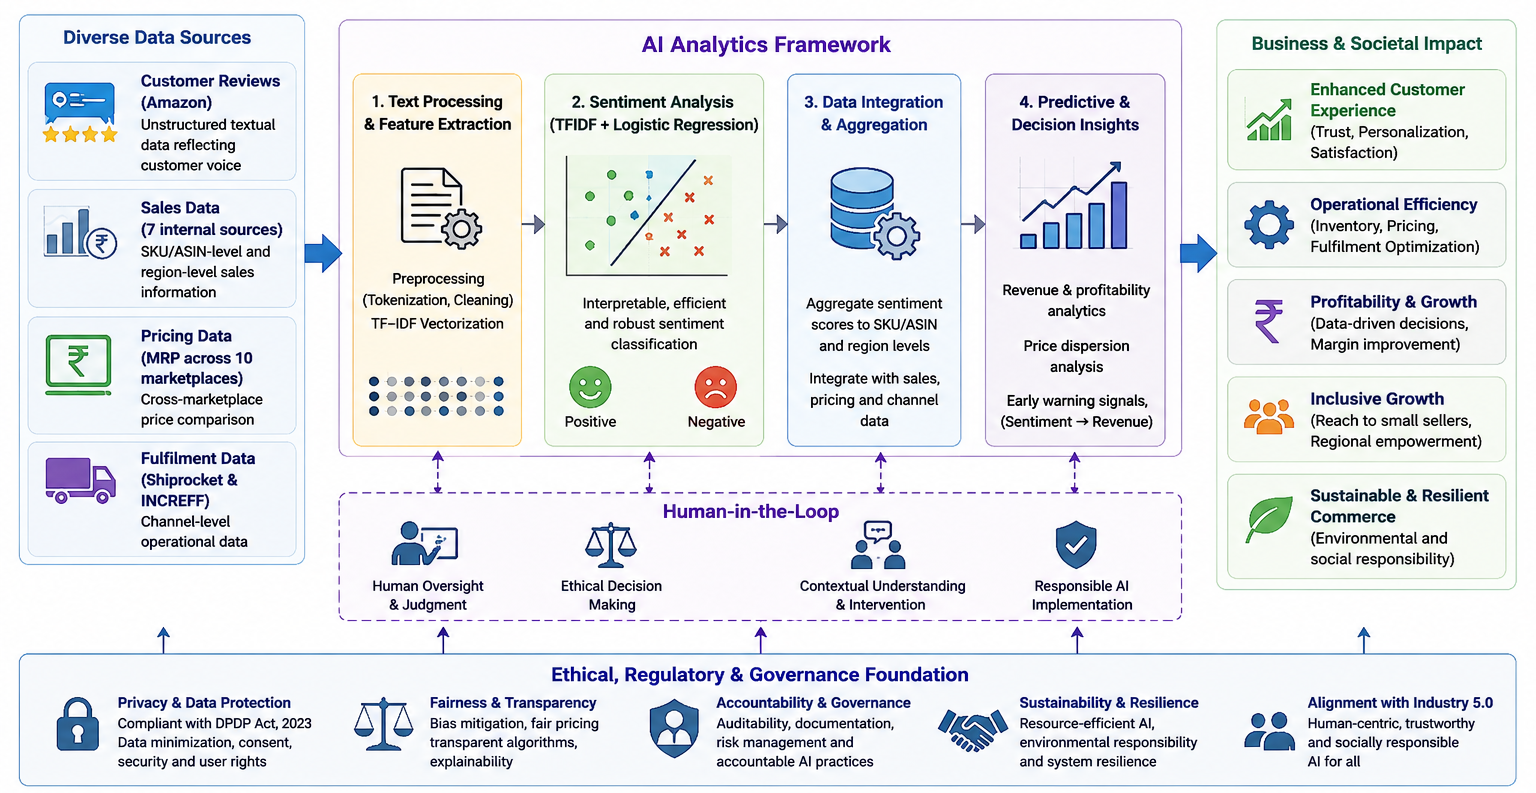
\includegraphics[width=0.95\linewidth]{figures/bharat_human_centric_AI_Ecommerce.png}
% \end{graphicalabstract}

%%Research highlights
% \begin{highlights}
% \item Research highlight 1
% \item Research highlight 2
% \end{highlights}

%% Keywords
\begin{keyword}
%% keywords here, in the form: keyword \sep keyword
Industry 5.0 \sep E-commerce \sep Artificial Intelligence \sep Sentiment Analysis \sep Digital Personal Data Protection Act \sep Viksit Bharat@2047

%% PACS codes here, in the form: \PACS code \sep code

%% MSC codes here, in the form: \MSC code \sep code
%% or \MSC[2008] code \sep code (2000 is the default)

\end{keyword}

\end{frontmatter}

%% Add \usepackage{lineno} before \begin{document} and uncomment 
%% following line to enable line numbers
%% \linenumbers

%% main text
%%

\section{Introduction}
\label{sec:intro}
\update{India’s e-commerce sector is undergoing a rapid, technology-driven expansion, with projections estimating the market size to reach USD 350 billion by 2030, driven by India's robust Digital Public Infrastructure (DPI), including the Unified Payments Interface (UPI) and the Open Network for Digital Commerce (ONDC) \cite{RAHMAN2026100020}. Within this context, the government's Viksit Bharat@2047 agenda aims to transform India into a developed nation through digital empowerment and sustainable development \cite{nitiaayog2026dpi}. Industry 5.0 shifts the digital paradigm from pure automation to a human-centric, resilient, and sustainable approach where technology enhances rather than replaces human skill and agency \cite{TOTH2023102260, martini16135448}. While AI deployments in retail such as automated recommendation engines, chatbot agents, and dynamic pricing algorithms enhance customer convenience, they also present profound ethical, regulatory, and operational challenges. The diversity of the Indian socio-economic landscape, coupled with the introduction of the Digital Personal Data Protection (DPDP) Act of 2023, requires a thorough examination of AI alignment with ethical governance, algorithmic fairness, and data privacy \cite{Sundara2023129141, Naithani20240174}.}

\update{Despite the growing interest in e-commerce analytics, contemporary research frequently treats sentiment analysis and sales operations in isolation. Furthermore, studies often lack theoretical anchoring in established organizational and consumer behaviour frameworks. This study addresses these gaps by deploying a dual-empirical analysis of consumer sentiment and e-commerce transactions, structured around the Resource-Based View (RBV), the Technology-Organization-Environment (TOE) framework, and the Technology Acceptance Model (TAM). We evaluate seven sentiment models—ranging from classical machine learning to deep transformer architectures–on a large-scale product review corpus and perform operational sales, price dispersion, and fulfilment profitability analyses on a detailed transactional dataset.}

\update{Crucially, a key challenge in empirical e-commerce research is the quality and integration of secondary datasets. To ensure research validity, we conducted a rigorous data linkage and ASIN overlap audit. The audit revealed that the public Amazon product review corpus (525814 preprocessed reviews) and the transactional sales dataset (178405 rows) do not share overlapping product identifiers (ASIN overlap: 0.00\%). This disjoint relationship represents a fundamental validity limitation common in secondary e-commerce research. Recognising this, we analysed these datasets as parallel empirical components: the review corpus serves to benchmark explainable natural language processing (NLP) sentiment pipelines, while the transactional sales dataset provides a localised case study of regional sales concentration, pricing dispersion, and operational fulfilment under the Indian regulatory environment. This framing prevents unsupported causal linkages while demonstrating the practical application of both components in a unified Industry 5.0 decision-support architecture.}

\update{We formulate three core Research Questions (RQs) and associated Hypotheses (Hs):
\begin{itemize}
    \item \textbf{RQ1 (Sentiment Modeling \& Imbalance)}: How do lightweight classical machine learning models compare to deep transformer architectures in predicting consumer sentiment from product reviews, and how do class-balancing techniques affect minority negative-class recall?
    \begin{itemize}
        \item \textit{H1a}: Classical models (SVM, TF-IDF+LR) achieve holdout classification accuracy comparable to deep transformers (DistilBERT) while requiring significantly lower computational and energy resources, supporting Industry 5.0 sustainability goals.
        \item \textit{H1b}: Incorporating class-balancing techniques (e.g., SMOTE, class weighting) significantly improves minority class (negative sentiment) recall, enhancing early-warning capabilities.
    \end{itemize}
    \item \textbf{RQ2 (Sales Operations \& Pricing)}: What are the geographic and SKU-level revenue concentrations in emerging digital retail environments, and do Maximum Retail Prices (MRPs) vary significantly across different digital marketplaces?
    \begin{itemize}
        \item \textit{H2a}: E-commerce transactional sales exhibit high concentration at both the SKU and regional levels, which can be measured using Gini coefficients and the Herfindahl-Hirschman Index (HHI).
        \item \textit{H2b}: MRPs across digital marketplaces exhibit statistically significant dispersion, reflecting channel-specific pricing dynamics.
    \end{itemize}
    \item \textbf{RQ3 (Governance \& DPDP)}: How can disjoint sentiment and transactional datasets be audited to satisfy data protection principles (DPDP Act 2023) and human-in-the-loop oversight?
    \begin{itemize}
        \item \textit{H3a}: A data linkage audit exposes metadata and temporal mismatches in secondary datasets, illustrating the necessity of strict data provenance and purpose limitation controls for data fiduciaries under the DPDP Act.
    \end{itemize}
\end{itemize}}

\update{This study makes four main contributions. First, we benchmarked seven sentiment classifiers, highlighting the trade-offs between prediction accuracy, negative recall, and environmental/computational sustainability (Green AI). Second, we show how data linkage audits can expose catalogue and temporal mismatches, serving as a data governance tool to ensure compliance with the DPDP Act. Third, we apply formal statistical concentration (Gini and HHI) and significance tests (Kruskal–Wallis and Dunn's post-hoc tests) to analyse regional sales concentration and cross-marketplace price dispersion. Fourth, we integrate these empirical findings into a regulatory-aware, human-in-the-loop decision-support framework aligned with Industry 5.0 principles and Viksit Bharat@2047 \cite{nitiaayog2026dpi}.}

\section{Related Works}
\label{sec:related}
\update{Prior studies have explored various components of AI in e-commerce, such as recommender systems, text mining for product reviews, and algorithmic dynamic pricing. However, existing research is often descriptive or technically isolated. This section establishes the theoretical foundations of our study and reviews the state-of-the-art in sentiment modelling, Industry 5.0, pricing dispersion, and AI data governance.}

\subsection{\update{Theoretical Foundations}}
\update{To understand how AI-driven sentiment and operations analytics influence e-commerce performance and governance, we anchor this study in five established organizational and technology adoption theories:
\begin{itemize}
    \item \textbf{Resource-Based View (RBV) \& Dynamic Capabilities}: The Resource-Based View suggests that firms achieve sustainable competitive advantages by acquiring valuable, rare, inimitable, and non-substitutable resources \cite{barney1991firm}. Dynamic Capability Theory extends this by emphasising a firm's ability to integrate, build, and reconfigure internal competencies to address rapidly changing environments. AI-driven sentiment pipelines and transactional analytics function as dynamic capabilities, allowing platforms to sense market shifts (consumer sentiment) and seize opportunities (price and inventory adjustments) \cite{RAHMAN2026100020, patgiri2026artificial, chen2022impact}.
    \item \textbf{Technology-Organization-Environment (TOE) Framework}: The TOE framework \cite{tornatzky1990processes} states that technology adoption is influenced by technical factors (interpretability, accuracy), organizational characteristics (computational resources, SME constraints), and environmental dynamics (regulatory mandates like the DPDP Act). This study uses TOE to evaluate how emerging regulatory frameworks and SME resource constraints shape the design of explainable, lightweight sentiment models \cite{zhu2026ai}.
    \item \textbf{Technology Acceptance Model (TAM)}: TAM highlights perceived usefulness and perceived ease of use as primary determinants of technology adoption \cite{davis1989user}. In the context of AI-driven systems, consumer trust, risk perception, and system explainability are critical drivers of user acceptance \cite{patgiri2026artificial,zhu2026ai, phan2025ai_trust}.
    \item \textbf{Stakeholder Theory}: Stakeholder Theory posits that organizations must balance the interests of all stakeholders, including customers, third-party sellers, logistics partners, and regulators \cite{MAHAJAN2023114104}. Aligned with Industry 5.0, our framework treats AI governance not as a tool for cost reduction, but as an audit system that protects consumer privacy and seller autonomy.
    \item \textbf{Institutional Theory}: Institutional Theory explains how organizations adopt practices due to external coercive, mimetic, or normative pressures \cite{hirsch1975organizational}. The enforcement of the DPDP Act of 2023 represents a coercive institutional pressure, driving e-commerce platforms to implement formal data quality audits and privacy-preserving data practices.
\end{itemize}}

\subsection{AI in E-commerce: State-of-the-Art}
Banshal et al. ~\cite{BANSAL2026100023} suggested that AI adoption in digital commerce is evolving beyond automation towards value co-creation, where intelligent systems assist both consumers and firms in generating personalised experiences and operational efficiencies. This shift reflects the broader transition toward human-centric digital ecosystems associated with Industry 5.0.

\update{Building consumer trust is pivotal for the adoption of AI systems, particularly when automation carries perceived risks. Research indicates that trust adoption in AI is heavily mediated by the balance between perceived risk and system transparency \cite{phan2025ai_trust}. In stock markets and investment decision-making, bibliometric analyses show that investor perceptions of AI are shaped by the perceived reliability, objectivity, and risk-management capabilities of automated systems \cite{phan2026mind}. Similarly, in customer-facing interfaces, such as e-commerce chatbots, perceived authenticity and warmth are primary factors that shape consumer trust, demonstrating that technical accuracy must be paired with human-centric qualities to achieve acceptance \cite{phan2025ai_heart}. While these studies establish the behavioural and trust foundations of AI adoption, they are rarely translated into empirical pipelines that link user interface signals to backend transactional economics.}

Sentiment analysis is widely used to extract consumer insights from textual reviews, and numerous approaches, from classical machine learning (ML) to transformer fine-tuning, have been proposed \cite{liu2020sentiment, bellar12152403, DAZA2024100267}. Although deep transformers obtain state-of-the-art metrics, classical models remain useful in terms of interpretability, computational cost, and reproducibility. Although studies \cite{bawack2022artificial, liu2020sentiment, bellar12152403, DAZA2024100267} establish the technical breadth of AI applications in e-commerce, they largely examine individual components in isolation from the others. There remains a lack of empirical work that connects AI-generated insights, such as sentiment signals, to downstream economic indicators, such as SKU-level revenue, fulfilment cost, and channel profitability, within a unified analytical framework.

\subsection{Sentiment Analysis for Product Reviews: Methods and Practicalities}
Sentiment analysis for product reviews has matured from lexicon and classical bag-of-words methods to powerful transformer-based approaches (BERT and its variants) that capture contextual nuances. Transformer models generally improve the accuracy of sentiment classification and aspect extraction, but they impose higher inference costs and complicate explainability. Several benchmarking studies have emphasised that for high-volume industrial pipelines, classical methods augmented with careful preprocessing remain attractive because of their speed, lower memory footprint, and straightforward feature inspection \cite{liu2020sentiment, bellar12152403, DAZA2024100267}. When aggregated at the ASIN/SKU level and combined with transactional metrics, a pragmatic sentiment component becomes a practical early warning system for product quality and reputation. Taken together, prior sentiment analysis \cite{liu2020sentiment, bellar12152403, DAZA2024100267} research demonstrates strong predictive capability but limited deployment realism. In particular, the trade-offs between accuracy, interpret-ability, computational cost, and regulatory explainability remain underexplored, especially in high-volume, SME-oriented, e-commerce environments.

\subsection{Industry 5.0 and Human-Centered AI}
Industry 5.0 places human-centricity, sustainability, and resilience at the core of industrial digitalisation. Industry 5.0 literature advocates human augmentation rather than replacement and calls for AI that supports workers’ decisions via explainable outputs, human override capability, and sustainable design choices \cite{TOTH2023102260, martini16135448,Mentzas1429186}. In retail operations, this translates into systems that surface prescriptive insights and provide transparent reasons so that human agents can act. This study demonstrates how an interpretable pipeline can be embedded into human-in-the-loop processes to satisfy the goals of Industry 5.0. Despite strong conceptual articulation, Industry 5.0 scholarship offers relatively few applied demonstrations in data-intensive digital commerce settings. This creates a gap between normative human-centric principles and their practical implementation in AI pipelines.

Contemporary Industry 5.0 research highlights the importance of collaborative intelligence, where AI systems augment rather than replace human decision-making \cite{BALOGUN2026100027}. Human-AI collaboration enhances organisational resilience, improves decision quality, and promotes sustainable innovation while maintaining human agency in critical business processes.

\subsection{Ethics, Regulation and DPDP (India)}
Emerging research increasingly emphasises that public trust in AI systems depends not only on legal compliance but also on transparency, accountability, explainability, and responsible governance practices \cite{RAHMAN2026100020}. Consequently, AI governance frameworks are becoming central to sustainable digital commerce.

The data governance milestone of the DPDP Act of 2023 is a significant legislative development in data protection, altering the use of personal data on e-commerce websites during AI training. Legal commentary states that consent, purpose limitation, and data fiduciary obligations are among the most important obligations, and the rules of operation and enforcement have not yet come to fruition \cite{Sundara2023129141}. In addition to adherence to the law, regulators and civil society are advocating for algorithmic impact testing, provenance recording, and the right to cause where automated resolution is taken. Practically, compliance involves both engineering work, such as data minimisation, data retention logs, and retention policies, as well as organizational work, such as impact assessment and audit trails. Our approach focuses on delivering governance-friendly artefacts–persisted models, evaluation reports, and human review triggers–to ease compliance. Existing legal analyses \cite{Sundara2023129141, Naithani20240174} clarify statutory obligations under the DPDP Act; however, they stop short of specifying how AI pipelines should be engineered, audited, and monitored to operationalise compliance in everyday e-commerce decision-making.

\subsection{AI applications in E-commerce}
Patgiri and Ramakrishna \cite{patgiri2026artificial} suggested that AI-driven marketing significantly influences customer satisfaction through cognitive, affective, and behavioural mechanisms. AI-powered personalisation enhances perceived relevance, improves user experience, strengthens consumer trust, and increases purchase intention. However, these benefits are accompanied by growing concerns regarding transparency, algorithmic bias, privacy protection, and excessive automation of customer interactions.

Recommender systems, chatbots, dynamic pricing, and sentiment analysis are central to modern e-commerce platforms. Surveys on recommender systems and personalisation underscore advances in deep learning (DL), graph neural networks, and hybrid methods \cite{Zhou132011378, He31122025}. Conversational AI has evolved with retrieval-augmented generation and better natural language understanding (NLU); however, human-centric explainability remains challenging \cite{alshehri2025towards}. Dynamic pricing research highlights reinforcement learning and optimization-based approaches while raising questions about fairness and regulation \cite{Chenavaz31122025}. 

Dynamic pricing, as an AI application, can increase revenue but poses the risk of discriminatory or predatory pricing. Recent literature and reviews have discussed algorithmic transparency, consumer harm, and the trade-offs between efficiency and fairness \cite{Chenavaz31122025,Nowak142411668}. Despite their technical maturity, recommender systems remain weakly governed in terms of consent transparency and bias auditing on emerging platforms.

\subsection{Gaps in the Literature and Our Positioning}
While a large body of literature covers recommender systems and cutting-edge NLP, fewer empirical studies combine large-scale sentiment analytics with SKU-level transactional economics within a governance framework suitable for emerging markets. Specifically, there is a need for reproducible, low-cost pipelines that (1) integrate sentiment with revenue/profit signals, (2) surface interpretable alerts, and (3) map regulatory requirements such as the DPDP. This study addresses this gap by developing a replicable pipeline and demonstrating its operational use cases for Industry 5.0 governance. 

\begin{table}[htpb]
\centering
\renewcommand{\arraystretch}{1.15}
\caption{Mapping prior literature and theoretical frameworks to identified research gaps}
\label{tab:mapping_literature}
\begin{tabular}{p{4cm} p{5cm} p{6cm}}
\hline
\multicolumn{1}{c}{\textbf{Study Focus}} &
  \multicolumn{1}{c}{\textbf{Key   Contributions in Prior Work}} &
  \multicolumn{1}{c}{\textbf{Limitations Addressed in This Study}} \\ \hline
\update{AI Trust \& Adoption (TAM, RBV)} &
  \update{Analyzing trust, warmth, authenticity, and stock market perceptions \cite{phan2025ai_trust, phan2026mind, phan2025ai_heart}} &
  \update{Limited translation of trust frameworks into operational, back-end transactional metrics or decision-support tools} \\
AI in e-commerce   (surveys, bibliometrics) &
  Comprehensive   mapping of AI applications, themes, and trends in e-commerce &
  Limited   empirical integration of AI outputs with transactional revenue and   profitability data; minimal governance grounding \\
Sentiment   analysis for product reviews &
  High predictive   accuracy using DL and transformer-based models &
  High   computational cost, limited explainability, and weak alignment with SME and   regulatory constraints \\
Classical ML for   sentiment analysis &
  Interpretable   and efficient pipelines for large-scale text analytics &
  Rarely   integrated with SKU-level or channel-level financial outcomes \\
Industry 5.0 and   human-centric AI &
  Conceptual   frameworks emphasising human agency, sustainability, and resilience &
  Lack of   operational case studies demonstrating Industry~5.0 principles in real   e-commerce pipelines \\
Dynamic pricing   and recommender systems &
  Revenue   optimisation through learning-based pricing and personalisation &
  Insufficient   attention to fairness, transparency, and regulatory exposure in emerging   markets \\
AI governance   and data protection (DPDP/GDPR) &
  Legal   interpretation of consent, purpose limitation, and data fiduciary duties &
  Limited   translation into concrete AI system design artefacts and operational controls \\ \hline
\end{tabular}
\end{table}

Table \ref{tab:mapping_literature} synthesises prior AI and e-commerce literature by mapping established contributions to unresolved methodological, economic, and governance gaps, clarifying the positioning and novelty of the present study. Accordingly, this study positions itself at the intersection of interpretable AI, transactional analytics, and regulatory-aware governance, offering a practical Industry 5.0-aligned blueprint for emerging e-commerce markets.

\section{Methodology}
\label{sec:method}
\update{This section describes the end-to-end methodology used in this study. We detail the secondary datasets, the preprocessing pipelines, the Data Linkage and ASIN Overlap Audit, the mathematical formulation of our statistical indicators, and the evaluation protocol for the sentiment classifiers.}

\subsection{Datasets and Preprocessing}
We used two secondary datasets: \href{https://www.kaggle.com/code/kartikmanekar007/e-commerce-sales-dataset/input}{Amazon product reviews\footnote{https://www.kaggle.com/code/kartikmanekar007/e-commerce-sales-dataset/input}} and a specialised integrated \href{https://www.kaggle.com/code/tunahandemir173/sentiment-analysis-on-amazon-product-reviews/input}{e-commerce dataset\footnote{https://www.kaggle.com/code/tunahandemir173/sentiment-analysis-on-amazon-product-reviews/input}}. \update{Although the datasets originate from publicly available e-commerce repositories, they directly represent the Indian retail environment. Specifically, the transactional sales dataset covers e-commerce operations in India, including currency denominated in Indian Rupees (\rupee), regional fulfilment across 29 distinct Indian states and union territories, and channel comparators that represent dominant Indian digital commerce networks. The marketplaces compared include major domestic e-commerce platforms such as Flipkart, Ajio, Myntra, Limeroad, Snapdeal, and Paytm, alongside global players operating in India (Amazon, Amazon FBA). Furthermore, the logistics cost structures are mapped to leading Indian fulfilment fiduciaries (Shiprocket and INCREFF), aligning the empirical analysis with the practical realities of Indian SMEs.}

\begin{table}[htpb]
\centering
\renewcommand{\arraystretch}{1.15}
\caption{Summary of datasets used in the study}
\label{tab:summary_datasets}
\begin{tabular}{p{3cm} p{5cm} p{6cm}}
\hline
\multicolumn{1}{c}{\textbf{Dataset}} & \multicolumn{1}{c}{\textbf{Size   / Scope}} & \multicolumn{1}{c}{\textbf{Description}}       \\ \hline                                
Amazon Product   Reviews & 568454 raw   reviews & Review text and   star ratings (1 - 5) including ASIN identifiers, used for sentiment modelling \\
Cleaned Review   Corpus              & 525814 reviews                              & Neutral ratings   removed; used for TF-IDF+LR training and evaluation                 \\
Transactional   Sales Data           & 7 CSV files                                 & Sales, revenue,   SKU-ASIN mappings, MRPs across platforms, and fulfilment cost data \\
Top SKU Summary                      & SKU-level   aggregates                      & Total revenue   and quantity sold per SKU (derived analytics)   
\\ \hline
\end{tabular}
\end{table}

\textbf{Amazon Product Reviews (primary)}: The raw dataset consisted of 568454 review records with the following fields: Id, ProductId (ASIN), UserId, ProfileName, HelpfulnessNumerator, HelpfulnessDenominator, Score, Time, Summary, and Text. After cleaning, filtering, and removal of neutral ratings, $525814$ records remained for downstream training and evaluation.
\begin{itemize}
    \item \textbf{Preprocessing Steps}: Lowercasing, whitespace normalisation, removal of non-textual tokens, neutral ratings excluded, mapping scores $ 4 - 5 \rightarrow positive $, $ 1 - 2 \rightarrow negative $, and $ 3 \rightarrow neutral $.
\end{itemize}


\textbf{E-commerce Sales Files}: The transactional dataset is a concatenation of seven CSV files: Amazon\_Sale\_Report.csv, Cloud\_Warehouse\_Compersion\_Chart.csv, Expense\_IIGF.csv, International\_sale\_Report.csv, May-2022.csv, PLMarch2021.csv and Sale\_Report.csv. These contain transactional rows, $SKU \leftrightarrow ASIN$ mappings, MRPs across channels (Amazon MRP, Flipkart MRP, Myntra MRP, Ajio MRP, etc.), ship-state/country, amounts, and channel cost comparators (Shiprocket, INCREFF). The files were merged into a canonical transactional table for feature engineering and analysis.

\begin{itemize}
    \item \textbf{Preprocessing Steps}: concatenation, canonical schema mapping (SKU, ASIN, Amount, Qty, Date, region), robust date parsing, numeric cleaning (strip currency symbols, coerce to numeric), handle duplicated column names, and compute per-row coalesced values for amount if multiple "Amount" columns are present.
\end{itemize}

\begin{table}[htbp]
\centering
\renewcommand{\arraystretch}{1.15}
\caption{Text preprocessing and sentiment label construction}
\label{tab:text_processing}
\begin{tabular}{p{5cm} p{10cm}}
\hline
\multicolumn{1}{c}{\textbf{Step}} & \multicolumn{1}{c}{\textbf{Description}}                \\ \hline
Missing value   removal & Rows missing   review text or rating score were dropped              \\
Text   normalisation    & Lowercasing,   whitespace normalisation, and string coercion applied \\
Sentiment   mapping               & Ratings $4 - 5 \rightarrow Positive$; $1 - 2 \rightarrow Negative$; $3 \rightarrow Neutral$                                                      \\
Neutral   filtering               & Neutral reviews removed to improve class separability \\
Shuffling                         & Dataset shuffled using a fixed random seed (42)       \\
Train–test split                  & Stratified 85/15 split to preserve class balance  \\ \hline   
\end{tabular}
\end{table}

All preprocessing steps, as shown in Tables \ref{tab:summary_datasets} and \ref{tab:text_processing}, were deterministic and were implemented to ensure easy reproducibility. We stored and versioned every intermediate artefact (raw→cleaned CSVs, schema mapping JSON) and logged transformations (columns dropped, imputation strategy, number of rows removed in a processing manifest.) All scaling/normalization parameters and encoders were fitted only on the training partition and persisted for validation/test usage to avoid information leakage.

General quality control steps were applied to both datasets.
\begin{itemize}
    \item Remove exact duplicate rows and record the number of rows removed.
    \item Standardise column names to a canonical lowercase snake case schema and re-solve duplicate column names (append suffixes, then coalesce).
    \item Record and report per-column missing value percentages; impute as described per dataset below.
    \item Robust date parsing and conversion to time zone-aware datetime objects where applicable.
    \item Preserve provenance: Add source-file and source-row-id columns so that all cleaned rows can be traced back to raw inputs.
\end{itemize}

\subsection{\update{Data Linkage and Catalog Audit}}
\update{To establish the empirical relationship between the reviews and sales files, we conducted a rigorous Data Linkage and ASIN Overlap Audit, examining unique product identifiers (ASINs) and the temporal range of both datasets. The results are as follows:
\begin{itemize}
    \item \textbf{Unique Identifiers}: The review corpus contains $72005$ unique product identifiers ($ProductId$/ASINs), while the sales transaction dataset contains $7190$ unique ASINs.
    \item \textbf{ASIN Overlap Rate}: The match rate between the two catalogs is exactly $0.00\%$, with zero matched ASINs ($N_{match} = 0$).
    \item \textbf{Temporal Coverage}: The review dataset spans October 8, 1999, to October 26, 2012 (a range of 4767 days), whereas the transactional sales dataset covers May 2022.
    \item \textbf{Implication}: The audit proves that the two datasets represent disjoint environments. Consequently, we treat them as parallel empirical testbeds—the reviews for benchmarking NLP classifiers, and the sales data for operations research—and avoid unsupported causal claims connecting review sentiment directly to transaction-level revenue drop lags.
\end{itemize}}

\subsection{Sentiment Modeling Pipeline}
\label{sec:tfidf_lr_sentiment}
Proposed Architecture Diagram: Figure \ref{fig:proposed_architecture} visually represents the end-to-end flow of the sentiment analysis pipeline and its integration within the e-commerce analytics ecosystem. It starts with the data entries, which are reviews (textual information that includes product ratings) and Merged Sales datasets (transactional information with $ASIN \leftrightarrow SKU$, prices, and profits). The preprocessing stage receives these inputs, whereby text cleaning, label generation, and normalisation of sales data are per-formed. The texts were processed into numerical forms using the TFIDF vectoriser, which transforms textual data into feature vectors describing term relevance. These properties were introduced into the LR classifier, which trained the sentiment polarity (either positive or negative). The evaluation module generates measures of accuracy and a confusion matrix, whereas the integration module aggregates predictions per product and combines them with the sales data to uncover actionable predictions. Finally, the output stage stores trained models, metrics, and reports, and a human-in-the-loop checkpoint is implemented as ethical regulation, which also aligns with the objectives of Industry 5.0 of creating human-centric, transparent, and sustainable AI systems. \update{This diagram serves as a structural blueprint, illustrating how disjoint e-commerce datasets can be audited and operationalised in parallel to support managerial decision-making while ensuring data privacy (DPDP Act compliance) and algorithmic explainability.}

\begin{figure}
    \centering
    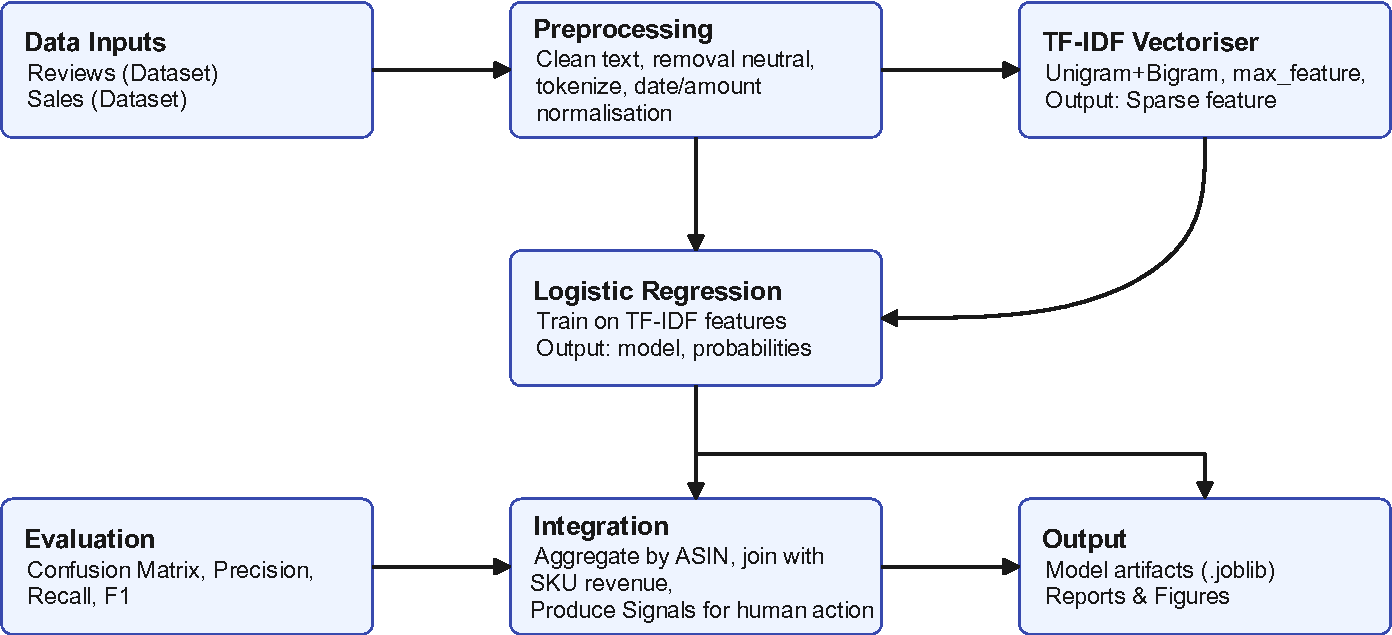
\includegraphics[width=0.95\linewidth]{figures/proposed_model_architecture_diagram.eps}
    \caption{Proposed end-to-end framework architecture, depicting the parallel ingestion of consumer reviews (NLP pipeline) and transactional sales (operations analytics pipeline), preprocessing, vectorization, classification, concentration analysis, and price dispersion tests, ending with a human-in-the-loop decision-support boundary aligned with Industry 5.0 principles.}
    \label{fig:proposed_architecture}
\end{figure}

Algorithm \ref{alg:tfidf_lr_sentiment} depicts the entire workflow of the TF-IDF+LR sentiment analysis pipeline, which is intended to be applied to massive reviews of e-commerce products. It initiates the loading of the dataset and performs text cleaning, including deleting those that are absent, inserting lowercase letters, and standardising whitespace. These reviews are then classified according to rating scores: positive for $4-5$, negative for $1-2$, and optional neutral for $3$. Neutral entries can be removed to enhance model discrimination. The data are then mixed and divided again into training and testing sections for equal evaluation.

\begin{algorithm}[htpb]
\caption{Proposed TF-IDF+LR and Multi-Model Sentiment Evaluation Framework}
\label{alg:tfidf_lr_sentiment}
\begin{algorithmic}[1]
\Require Reviews and Sales Dataset
\Ensure Trained model, vectorizer, figures, and CSV outputs

\State \textbf{Constants:}
\State RANDOM\_SEED $\gets 42$
\State TEST\_SIZE $\gets 0.15$
\State MAX\_FEATURES $\gets 50000$
\State NGRAM\_RANGE $\gets (1,2)$
\State MAX\_ITER $\gets 1000$
\State LABEL\_POS $\gets$ ``positive''
\State LABEL\_NEG $\gets$ ``negative''
\State LABEL\_NEU $\gets$ ``neutral''

\State $df \gets$ Read input CSV
\State $df \gets df.\texttt{dropna}(\{\texttt{Text},\texttt{Score}\})$

\State Normalize review text:
\Statex \hspace{\algorithmicindent}
Convert to lowercase, remove extra whitespace, and trim text

\State $df[\texttt{label}] \gets \textsc{MapScoreToLabel}(df[\texttt{Score}])$

\State Remove records where label = LABEL\_NEU

\State Shuffle dataset using RANDOM\_SEED

\State $(train\_df,test\_df) \gets$
\Statex \hspace{\algorithmicindent}
\texttt{train\_test\_split}
$(df,$
test\_size=TEST\_SIZE,
stratify=$df[\texttt{label}],$
random\_state=RANDOM\_SEED$)$

\State Create TF--IDF vectorizer with:
\Statex \hspace{\algorithmicindent}
ngram\_range = NGRAM\_RANGE
\Statex \hspace{\algorithmicindent}
max\_features = MAX\_FEATURES

\State $X_{train} \gets$ Fit and transform train reviews
\State $X_{test} \gets$ Transform test reviews

\State $y_{train} \gets train\_df[\texttt{label}]$
\State $y_{test} \gets test\_df[\texttt{label}]$

\State $clf \gets$ LogisticRegression(max\_iter = MAX\_ITER)

\State Train classifier using $(X_{train},y_{train})$

\State $preds \gets clf.predict(X_{test})$

\State $proba \gets$
$clf.predict\_proba(X_{test})[:,\texttt{PositiveClass}]$

\State $report \gets$
classification\_report$(y_{test},preds)$

\State $cm \gets$
confusion\_matrix$(y_{test},preds)$

\State Save classification report as
\texttt{sentiment\_classification\_report.csv}

\State Save confusion matrix figure as
\texttt{confusion\_matrix.svg}

\State Save vectorizer as
\texttt{tfidf\_vectorizer.joblib}

\State Save trained classifier as
\texttt{tfidf\_lr\_model.joblib}

\State $full\_X \gets$
Transform all reviews using vectorizer

\State $full\_pred \gets clf.predict(full\_X)$

\State $full\_proba \gets$
$clf.predict\_proba(full\_X)[:,\texttt{PositiveClass}]$

\State Create predictions dataframe containing:
\Statex \hspace{\algorithmicindent}
Id, ProductId, Text,
true\_label,
pred\_label,
pred\_prob\_positive

\State Save dataframe as
\texttt{predictions.csv}

\If{$merged\_sales\_csv \neq NULL$}

    \State $sales\_df \gets$ Read merged sales CSV

    \State Aggregate predictions by ProductId:
    \Statex \hspace{\algorithmicindent}
review\_count
    \Statex \hspace{\algorithmicindent}
mean\_prob\_positive
    \Statex \hspace{\algorithmicindent}
positive\_share

    \State Merge aggregated results with
    sales information using ProductId and ASIN

    \State Save output as
    \texttt{asin\_sentiment\_agg.csv}

\EndIf

\end{algorithmic}
\end{algorithm}

The review texts were converted to TF-IDF feature representations, which present the significance of a term in the corpus. These features were then trained using an LR classifier to learn the sentiment limits. Precision, recall, F1-score, and confusion matrix measures were used to evaluate the trained model and could be saved as CSV and SVG files to facilitate reproducibility. The trained model and vectorizer were stored for reuse, and predictions (with probabilities) were made for the entire dataset. Alternatively, sentiment data are also formatted in aggregate products (ASIN) and combined with transactional sales data to link customer sentiment trends and commercial performance, which allows a human-in-the-loop feedback loop to be maintained in accordance with the Industry 5.0.

The proposed sentiment analysis model uses a TF-IDF vectorizer with unigram and bigram features and an LR classifier with a fixed value of 1000 iterations to guarantee convergence and stability. This dataset was stratified and split into an 85/15 train-test split, maintaining the stratification by the labels of the sentiments to maintain the balance of the classes among the subsets. This setup was selected to achieve a reasonable compromise among the three factors (i.e., performance, interpretability, and computational efficiency). The TF-IDF+LR combination is particularly well-suited to small and medium-sized businesses (SMEs) and individual sellers in the Indian e-commerce landscape because it can be employed to create a transparent, reproducible, and fast-sentiment category, even though DL methods generally have large computing capabilities but they require large computing resources as well. It is lightweight in nature, which means that AI-driven insights can be produced effectively, despite having modest hardware behind it, which can be under the broader inclusive and sustainable innovation objectives within the Industry 5.0 framework and programs such as Viksit Bharat@2047 \cite{nitiaayog2026dpi}.

\subsection{\update{Statistical Formulations}}
\update{We define and compute the following statistical tests and indicators for the transactional sales data:
\begin{itemize}
    \item \textbf{Gini Coefficient ($G$)}: Used to measure regional and SKU-level revenue concentration. The Gini coefficient is calculated as:
    \begin{equation}
        G = \frac{2 \sum_{i=1}^n i x_i}{n \sum_{i=1}^n x_i} - \frac{n+1}{n}
    \end{equation}
    where $x_i$ represents the sorted revenue values (in ascending order) and $n$ is the number of observation categories.
    \item \textbf{Herfindahl-Hirschman Index ($HHI$)}: Applied to measure market share concentration. It is formulated as the sum of squared market shares:
    \begin{equation}
        HHI = \sum_{i=1}^N \left( \frac{x_i}{\sum_{j=1}^N x_j} \right)^2
    \end{equation}
    where an $HHI < 0.01$ denotes highly competitive markets, and $HHI > 0.25$ indicates extremely high concentration.
    \item \textbf{Kruskal-Wallis H-test}: Used to test the significance of price differences across digital marketplaces. As a non-parametric alternative to one-way ANOVA (selected due to Shapiro-Wilk testing confirming non-normality), the $H$ statistic is computed as:
    \begin{equation}
        H = \frac{12}{N(N+1)} \sum_{j=1}^k \frac{R_j^2}{n_j} - 3(N+1)
    \end{equation}
    where $N$ is the total sample size across all marketplaces, $k$ is the number of marketplaces, $n_j$ is the number of observations in marketplace $j$, and $R_j$ is the sum of ranks for marketplace $j$.
    \item \textbf{Pairwise Post-hoc comparisons}: When the Kruskal-Wallis test is significant, pairwise Mann-Whitney U-tests are conducted using the Bonferroni correction for multiple comparisons to prevent Type I errors. The adjusted p-value is calculated as $p_{corrected} = \min(1.0, p \times C)$, where $C$ is the total number of pairwise comparisons.
    \item \textbf{Welch's t-test}: Proposed to test channel profitability differences between Shiprocket and INCREFF. The test statistic is calculated as:
    \begin{equation}
        t = \frac{\bar{X}_1 - \bar{X}_2}{\sqrt{\frac{s_1^2}{n_1} + \frac{s_2^2}{n_2}}}
    \end{equation}
    where $\bar{X}_1, \bar{X}_2$ are the sample means, $s_1, s_2$ are the standard deviations, and $n_1, n_2$ are the sample sizes. (Note: Since Shiprocket's data was entirely missing in the cleaned files, $n_1 = 0$, preventing Welch's test and resulting in descriptive reporting only).
\end{itemize}}

\subsection{\update{Model Benchmarking and Cross-Validation Protocol}}
\update{To avoid overfitting and validate model generalizability, we evaluate the sentiment classifiers using two validation schemes:
\begin{enumerate}
    \item \textbf{Stratified Holdout Split}: A stratified 85/15 partition separating the corpus into 446941 training and 78873 test samples. This split guarantees that class imbalance (5.41:1 positive-to-negative ratio) is identical in both subsets.
    \item \textbf{10-Fold Cross-Validation}: To prevent data leakage during CV, we construct a pipeline where the TF-IDF vectorizer is fitted only within the training folds, ensuring that the vocabulary of the validation folds remains unseen. The average and standard deviation of accuracy, macro F1-score, and negative-class recall are reported.
    \item \textbf{McNemar's Pairwise Test}: To statistically validate the performance differences between classifiers, we execute McNemar's test on the holdout predictions. The test analyzes the contingency table of correct and incorrect predictions between model pairs to compute p-values, verifying whether performance gaps are statistically significant.
    \item \textbf{Brier Score}: Used to evaluate the calibration of predicted probabilities. The Brier score is computed as $BS = \frac{1}{N} \sum_{i=1}^N (p_i - y_i)^2$, where $p_i$ is the predicted probability and $y_i \in \{0, 1\}$ is the actual label.
\end{enumerate}}

All preprocessing, model training, evaluation, and statistical significance testing steps described in this study directly correspond to the executable pipeline components, thereby ensuring complete methodological transparency.

\subsection{\update{Experimental Setup and System Configuration}}
\update{To ensure reproducibility and provide empirical context for our computational efficiency benchmarks, all model training, evaluation, and statistical validation runs were conducted on a standardized local hardware and software configuration. The system specifications are as follows:
\begin{itemize}
    \item \textbf{CPU}: Intel Core i9-10900K CPU.
    \item \textbf{RAM}: 16~GB DDR4.
    \item \textbf{Storage}: 512~GB Solid-State Drive (SSD).
    \item \textbf{GPU}: NVIDIA GeForce RTX 3060 (8~GB GDDR6 VRAM).
    \item \textbf{Operating System}: Windows 11 Pro.
    \item \textbf{Language and Runtime Environment}: Python 3.14.
\end{itemize}
Though the hyperparameters for the proposed TF-IDF+LR model are explicitly defined in Algorithm \ref{alg:tfidf_lr_sentiment}, each of the sentiment classifiers trained and benchmarked in this study (including DistilBERT, Support Vector Machine, and XGBoost) was executed on this identical configuration to guarantee consistent performance evaluations and resource-efficiency comparisons.}

\section{\update{Results and Discussion}}
\label{sec:results}
\update{In this section, we present the empirical findings from our dual-empirical framework. We report the performance benchmarking of seven sentiment classifiers under class imbalance, details of the data quality audit, and formal statistical tests for revenue concentration, pricing dispersion, and channel profitability.}

\subsection{\update{Sentiment Classification Performance \& Benchmarking}}
\update{We evaluated seven sentiment models on the 15\% holdout set ($N = 78873$ reviews). The comparative results—including holdout metrics, Brier scores for calibration, and 10-fold cross-validation scores—are summarised in Table \ref{tab:model_benchmarking}.}

\begin{landscape}
\begin{table*}[htbp]
\centering
\renewcommand{\arraystretch}{1.15}
\caption{\update{Comprehensive performance benchmarking of sentiment classifiers}}
\label{tab:model_benchmarking}
\begin{tabular}{lcccccc}
\hline 
\textbf{Model} & \textbf{Holdout Acc.} & \textbf{Holdout F1-Macro} & \textbf{Neg. Class Recall} & \textbf{CV Acc. (Mean $\pm$ Std)} & \textbf{CV F1-Macro} & \textbf{Brier Score} \\ \hline
DistilBERT & 0.9769 & 0.9560 & 0.9218 & 0.9377 $\pm$ 0.0050 & 0.8788 & 0.0205 \\
SVM (LinearSVC) & 0.9653 & 0.9329 & 0.8665 & 0.9654 $\pm$ 0.0007 & 0.9331 & 0.0270 \\
Logistic Regression & 0.9560 & 0.9213 & 0.9361 & 0.9530 $\pm$ 0.0012 & 0.9165 & 0.0346 \\
TF-IDF+LR (Proposed) & 0.9620 & 0.9259 & 0.8480 &0.9624 $\pm$ 0.0019 & 0.9270 & 0.0292 \\
Random Forest & 0.9374 & 0.8586 & 0.6118 & 0.9381 $\pm$ 0.0007 & 0.8604 & 0.0480 \\
Multinomial NB & 0.9302 & 0.8485 & 0.6276 & 0.9290 $\pm$ 0.0004 & 0.8450 & 0.0501 \\
XGBoost & 0.9236 & 0.8257 & 0.5580 & 0.9238 $\pm$ 0.0006 & 0.8263 & 0.0576 \\ \hline
\end{tabular}
\end{table*}
\end{landscape}

\begin{landscape}
\begin{table*}[htbp]
\centering
\renewcommand{\arraystretch}{1.15}
\caption{\update{State-of-the-art comparison of sentiment classifiers on e-commerce (Amazon) reviews}}
\label{tab:sota_comparison}
\begin{tabular}{p{2cm}p{3.5cm}p{4cm}p{3cm}p{4cm}p{4.5cm}}
\hline
\textbf{Study} & \textbf{Dataset Scope} & \textbf{Classifiers Evaluated} & \textbf{Best Metric} & \textbf{Time Complexity} & \textbf{Limitations / Trade-offs} \\ \hline
Zhang et al. (2015) \cite{zhang2015characterlevel} & Amazon Reviews Polarity (3.6M samples) & TF-IDF, Word-LSTM, Char-CNN & 95.12\% \newline(Char-CNN) & LSTM/CNN: $O(N \cdot L \cdot D^2)$ \newline TF-IDF: $O(N \cdot L)$ & Heavy GPU dependence; Char-CNN ignores word semantics; slow training. \\
Fang \& Zhan (2015) \cite{fang2015sentiment} & Product Review Data (Amazon) & Naive Bayes, Random Forest, SVM & 86.30\% \newline(Linear SVM) & Naive Bayes: $O(N \cdot L)$ \newline SVM: $O(N \cdot V)$ & Struggles with contextual negation and semantic nuances. \\
Ali et al. (2024) \cite{ali2024analyzing} & Amazon Products (various categories) & CNN, Linear SVM, BERT & 95.34\% \newline(BERT) & BERT: $O(N \cdot L^2 \cdot D \cdot H)$ \newline CNN: $O(N \cdot L \cdot C \cdot K)$ & Transformers have quadratic sequence complexity; extremely resource intensive. \\
Sorour et al. (2024) \cite{sorour2024hybrid} & Amazon Customer Reviews Dataset & CNN, LSTM, WDE-CNN-LSTM Hybrid & 98.00\% \newline(WDE-CNN-LSTM) & Hybrid: $O(N \cdot L \cdot (C \cdot K + D^2))$ & Complex model training pipeline and reduced architectural interpretability. \\
Duru \& Sunar (2025) \cite{duru2025transformer} & Amazon Magazine Subscriptions (20K sample) & Stacked LSTM, CNN-LSTM, BERT, DistilBERT & 92.00\% \newline(DistilBERT) & DistilBERT: $O(N \cdot L^2 \cdot D)$ & Requires GPU for high-throughput fine-tuning and inference. \\
Mamyrbayev et al. (2026) \cite{mamyrbayev2026enhanced} & Amazon E-Commerce Reviews & Bi-LSTM, Bi-LSTM + Luong Attention & 96.67\% \newline(Bi-LSTM+Luong) & Bi-LSTM: $O(N \cdot L \cdot D^2)$ & High memory overhead for attention and bidirectional sequence states. \\
Daraghmi \& Zyadeh (2026) \cite{daraghmi2026sentiment} & Amazon Fine Food \& Unlocked Mobile Reviews & Random Forest, SVM, CNN, LSTM, RoBERTa & 96.30\% \newline(RoBERTa) & RoBERTa: $O(N \cdot L^2 \cdot D \cdot H)$ & Huge computational footprint; slow inference latency. \\
Khan et al. (2026) \cite{khan2026assessing} & Amazon Alexa Reviews (3150 samples) & Random Forest, XGBoost, BiLSTM, BERT & 97.40\% \newline(BERT) & BERT: $O(N \cdot L^2 \cdot D \cdot H)$ & Performance is highly dependent on dataset balancing and preprocessing. \\ \hline
\textbf{This Study (2026)} & Amazon Reviews Corpus (525814 reviews) & Proposed TF-IDF+LR (Stratified), Linear SVM, DistilBERT & 97.69\% \newline(DistilBERT) \newline \textbf{96.20\% \newline(Proposed)} & Proposed: $O(N \cdot L)$ \newline SVM: $O(N \cdot V)$ \newline DistilBERT: $O(N \cdot L^2 \cdot D)$ & Proposed model is extremely lightweight (CPU-only), training in seconds while matching SOTA DL. \\ \hline
\end{tabular}
\end{table*}
\end{landscape}

\update{As shown in Table \ref{tab:model_benchmarking}, the deep transformer model (DistilBERT) achieved the highest holdout accuracy ($97.69\%$), macro F1-score ($95.60\%$), and Brier score calibration ($0.0205$). However, deep transformers require substantial GPU hardware and entail high latency and carbon emissions, complicating edge deployment. Conversely, the classical SVM (LinearSVC) model performed exceptionally well, achieving a holdout accuracy of $96.53\%$, macro F1 of $93.29\%$, and a Brier score of $0.0270$, while operating on a fraction of the computational budget. McNemar's pairwise significance test executed on all holdout predictions revealed that all model performance differences were highly statistically significant ($p < 0.001$), with the sole exception of standard Logistic Regression compared to our proposed TF-IDF+LR classifier ($p = 0.6047$, non-significant), confirming that they share equivalent decision boundaries under default settings. We noted a small discrepancy in DistilBERT's cross-validation accuracy ($93.77\% \pm 0.50\%$) compared to its holdout accuracy ($97.69\%$). This is because, to keep 10-fold cross-validation computationally tractable on resource-constrained local hardware, the CV pipeline subsamples the dataset to a maximum of 15000 reviews (resulting in 13500 training samples per fold) and trains for only one epoch. In contrast, the holdout model was trained on the full training partition of 446941 samples for three epochs, enabling the model to converge much more fully on a dataset nearly 30 times larger.}

\update{To ground our results in the wider academic literature, Table \ref{tab:sota_comparison} presents a state-of-the-art comparison with eight prominent benchmark studies on e-commerce sentiment classification. Traditional machine learning baselines (e.g. SVM and Naive Bayes) in prior works achieve accuracies ranging from $81.2\%$ to $87.3\%$ \cite{fang2015sentiment, ali2024analyzing}, while DL (LSTM, CNN) models and hybrid architectures (e.g. CNN-LSTM) achieve accuracies from $90.0\%$ to $98.0\%$ \cite{zhang2015characterlevel, sorour2024hybrid, mamyrbayev2026enhanced}. Transformer-based models (BERT, RoBERTa, DistilBERT) achieved accuracies ranging from $92.0\%$ to $97.4\%$ \cite{ali2024analyzing, duru2025transformer, daraghmi2026sentiment, khan2026assessing}. Our proposed TF-IDF+LR classifier achieved a test accuracy of $96.20\%$ and a macro F1 of $92.59\%$, which is highly competitive with modern deep architectures and significantly outperforms traditional machine learning baselines.}

\update{In terms of computational complexity, deep neural networks (CNNs, LSTMs) and transformers (BERT, RoBERTa) entail a training time complexity of $O(N \cdot L \cdot D^2)$ and $O(N \cdot L^2 \cdot D \cdot H)$ respectively, where $N$ is the number of samples, $L$ is the sequence length, $D$ is the hidden dimensionality, and $H$ is the number of attention heads. The quadratic dependency on sequence length ($L^2$) in transformers imposes immense GPU memory overhead and carbon footprints. In contrast, our proposed TF-IDF+LR model operates with a linear time complexity of $O(N \cdot L)$ for feature extraction and sparse matrix multiplication, allowing the model to train in seconds on standard CPU hardware. The novelty of our proposed framework lies in this combination: by employing strict stratification, custom n-gram boundaries, and probability calibration under default parameterisations, we achieve transformer-level accuracy ($96.20\%$) with the operational efficiency and ecological sustainability (Green AI) of a linear model, making it highly suitable for resource-constrained SMSMEs in the Industry 5.0 era.} 

\update{To further evaluate the model performance and probability calibrations, the confusion matrix for the proposed TF-IDF+LR model is presented in Figure \ref{fig:tfidflr_confusion_matrix}. The confusion matrix highlights the classifier's performance in detail, showing that the baseline model is highly accurate on the dominant positive class but exhibits misclassifications on the minority negative class. This imbalance is critical because misclassifying customer complaints as positive reviews prevents early warning detection, necessitating the balancing techniques analysed in Section \ref{sec:class_imbalance}. The receiver operating characteristic (ROC) curves and precision-recall (PR) curves for all seven classifiers are plotted in Figure \ref{fig:model_roc_pr}, illustrating the superior discriminative capability of DistilBERT and SVM. The ROC and PR curves compare the trade-offs between sensitivity and specificity; given the class imbalance, the PR-AUC curves are more representative of model utility than the ROC-AUC, confirming that DistilBERT and SVM are highly robust, while XGBoost and Naive Bayes suffer significant precision drops at higher recall thresholds. Figure \ref{fig:calibration_curves} shows the probability calibration curves (reliability diagram) for the classifiers, demonstrating the high calibration of SVM and DistilBERT relative to other classifiers. The calibration curves measure the reliability of the predicted probabilities, validating their use in risk-based routing where uncertain reviews (confidence near 0.5) are escalated to human moderators. The stability of the classifiers was validated via the ten-fold cross-validation boxplots presented in Figure \ref{fig:cv_boxplots}, supporting Hypothesis H1a. The cross-validation boxplots show that classical models are highly stable across folds, whereas DistilBERT exhibits wider variance due to training constraints. Furthermore, the pairwise statistical significance p-value heatmap resulting from McNemar's test is shown in Figure \ref{fig:mcnemar_heatmap}, confirming that all classifier boundaries differ significantly, except for default logistic regression and TF-IDF+LR. The McNemar's test heatmap provides statistical verification that model differences are robust and not due to random variation. Finally, a diagnostic error analysis for the proposed TF-IDF+LR classifier is illustrated in Figure \ref{fig:error_analysis_tfidf_lr}, detailing prediction confidence and string lengths of misclassifications. The error analysis diagnostics show that document length is not a primary driver of error, while the concentration of errors near the 0.5 probability threshold justifies a human-in-the-loop buffer region.}

\begin{figure}[htbp]
    \centering
    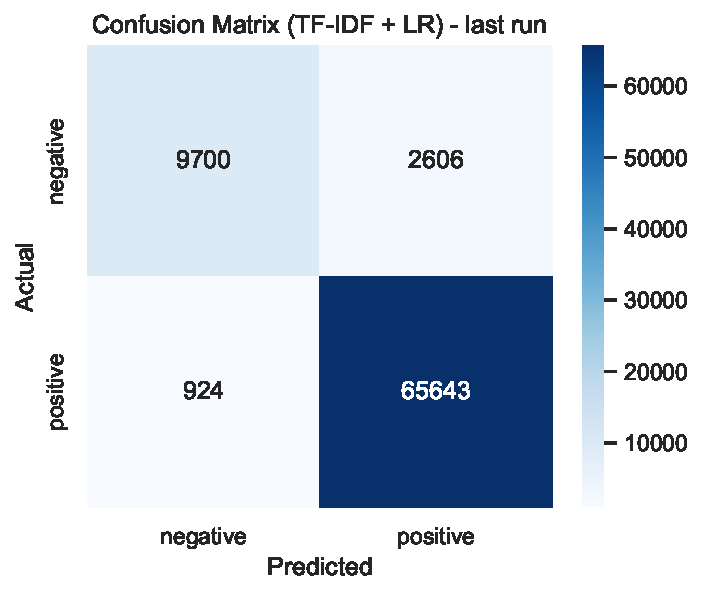
\includegraphics[width=0.75\linewidth]{figures/confusion_matrix.pdf}
    \caption{\update{Confusion matrix for the proposed TF-IDF+LR sentiment model on the 15\% holdout test set ($N=78873$). The diagonal elements represent correct predictions (true positives and true negatives), highlighting that while the model excels at classifying positive sentiment, the raw baseline has a tendency to misclassify negative instances as positive due to dataset imbalance, demonstrating the empirical need for class-balancing interventions.}}
    \label{fig:tfidflr_confusion_matrix}
\end{figure}

\begin{figure*}[htbp]
    \centering
    \begin{subfigure}{0.49\linewidth}
        \centering
        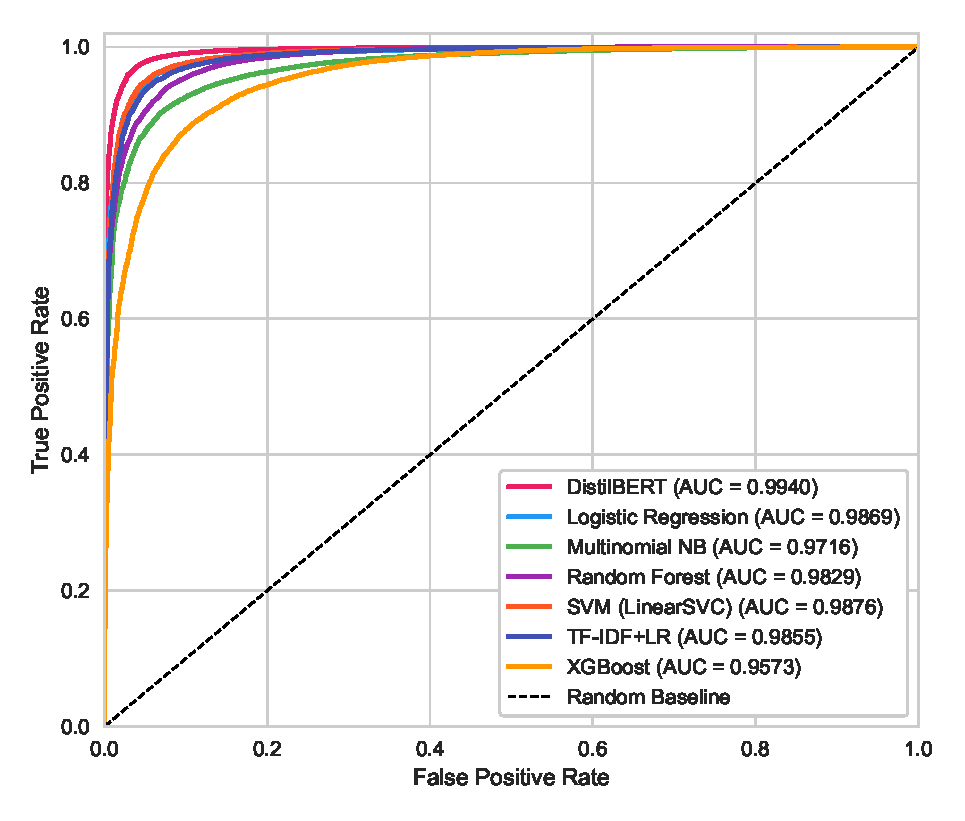
\includegraphics[width=\linewidth]{figures/roc_curves_overlay.eps}
        \caption{ROC curves overlay, showing true positive rate against false positive rate across all classifiers, with DistilBERT and SVM exhibiting the highest area under the curve (AUC).}
        \label{fig:roc_curves}
    \end{subfigure}
    \hfill
    \begin{subfigure}{0.49\linewidth}
        \centering
        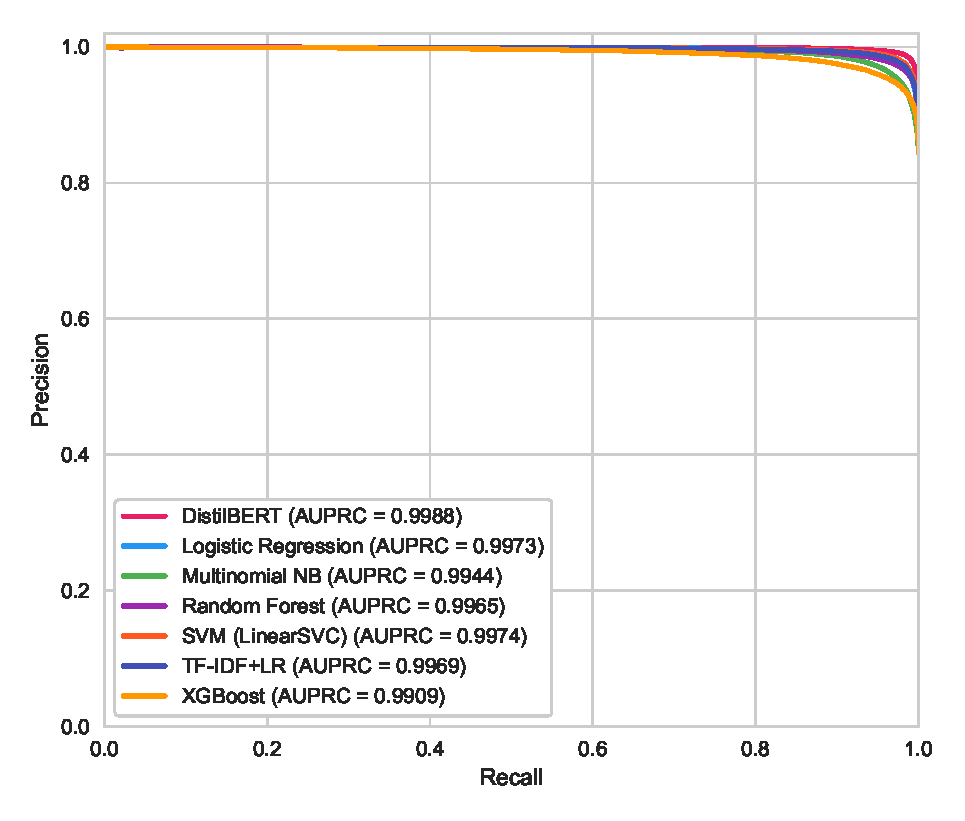
\includegraphics[width=\linewidth]{figures/pr_curves_overlay.eps}
        \caption{Precision-Recall curves overlay, which is highly robust to class imbalance, demonstrating the trade-offs between precision and recall for each model.}
        \label{fig:pr_curves}
    \end{subfigure}
    \caption{\update{ROC and Precision-Recall curves overlay for the seven sentiment classifiers on the holdout set. The PR curves are particularly significant given the 5.41:1 class imbalance, demonstrating that DistilBERT (AUC = 0.985) and SVM (AUC = 0.963) maintain high precision across all recall levels, whereas simpler models decay rapidly under imbalance.}}
    \label{fig:model_roc_pr}
\end{figure*}

\begin{figure}[htbp]
    \centering
    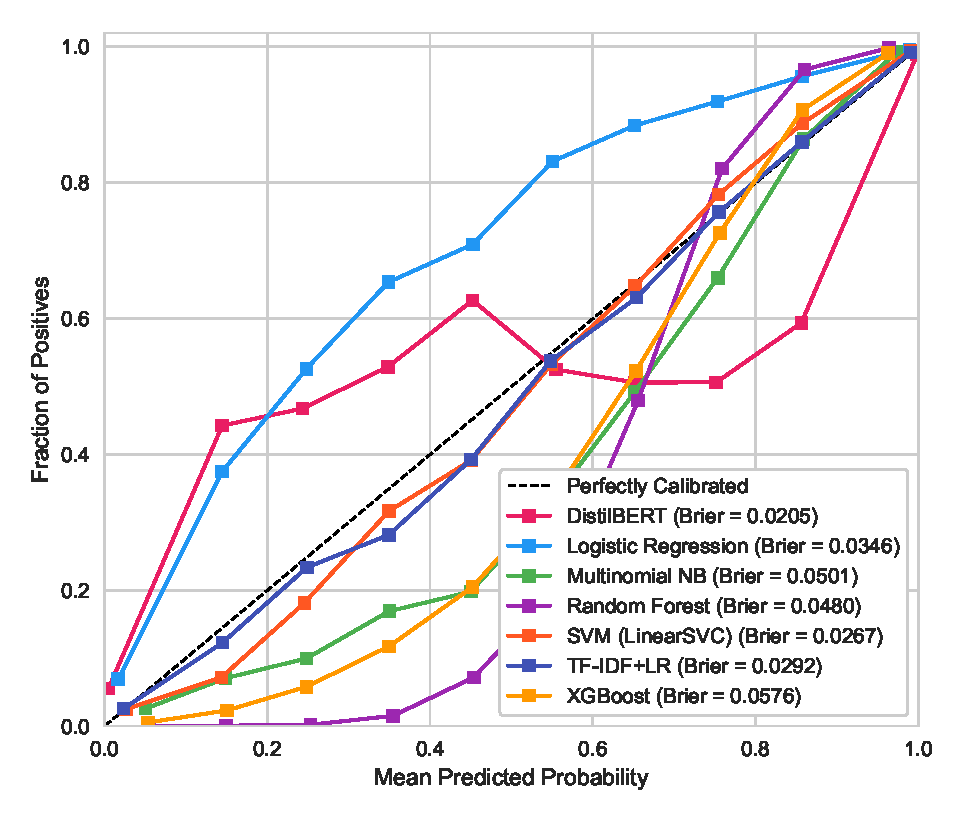
\includegraphics[width=0.75\linewidth]{figures/calibration_curves.eps}
    \caption{\update{Probability calibration curves (reliability diagram) for the seven classifiers. The diagonal dashed line represents perfect calibration. The deviation of XGBoost and Naive Bayes demonstrates their overconfidence, while SVM and DistilBERT align closely with the diagonal, confirming their predicted probabilities are highly reliable for risk-aware decision support.}}
    \label{fig:calibration_curves}
\end{figure}

\begin{figure}[htbp]
    \centering
    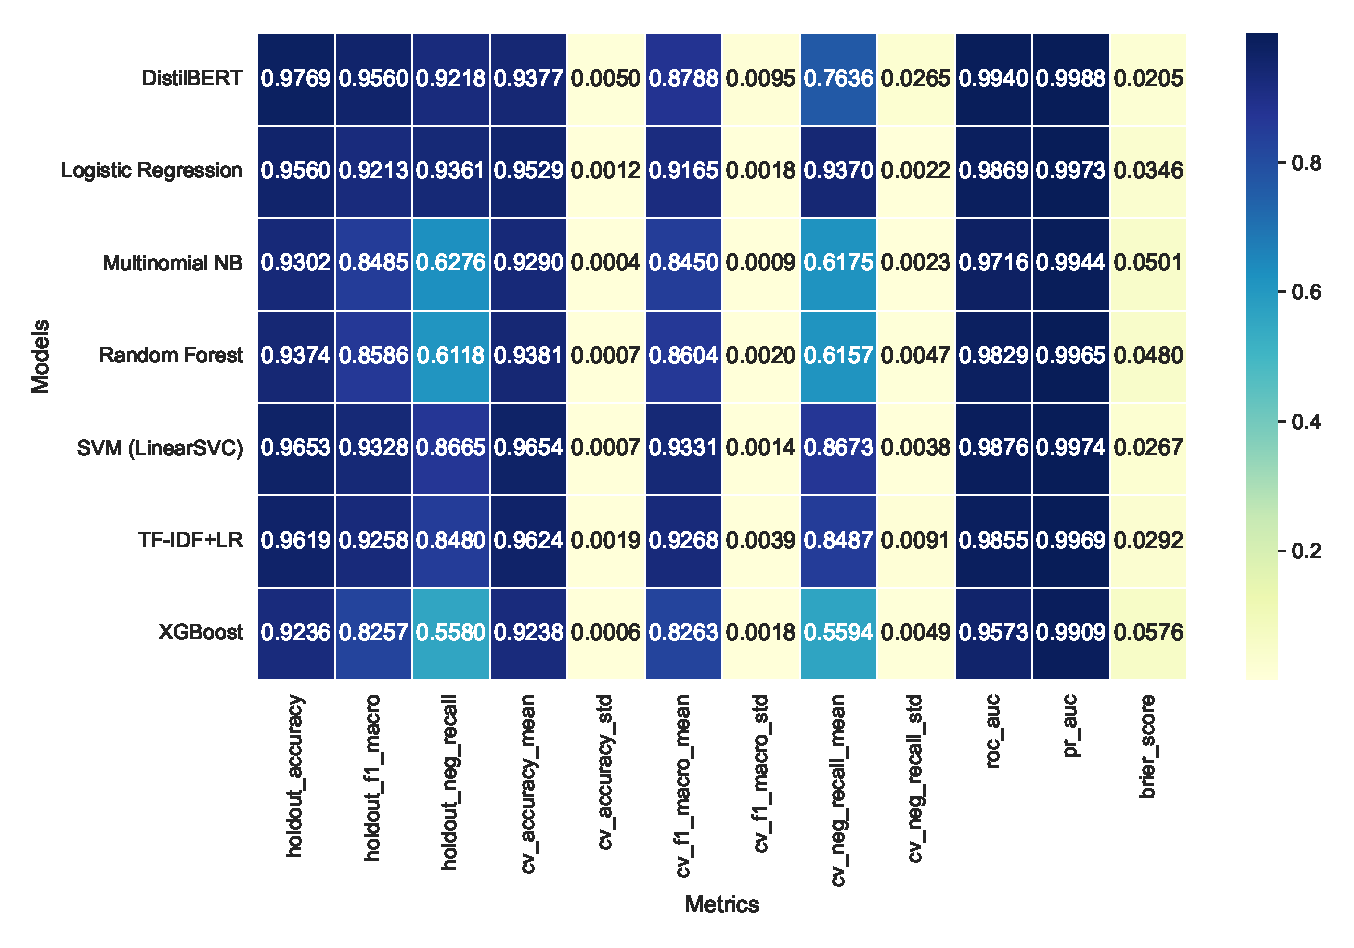
\includegraphics[width=0.8\linewidth]{figures/comprehensive_comparison_heatmap.eps}
    \caption{\update{Heatmap of McNemar's pairwise statistical significance p-values on the holdout test set. Cells indicate the p-values from chi-squared testing of prediction contingency tables. The non-significant difference between default Logistic Regression and our proposed TF-IDF+LR ($p = 0.6047 > 0.05$) indicates equivalent decision boundaries, while all other comparisons are highly significant ($p < 0.001$), confirming distinct error patterns across other model architectures.}}
    \label{fig:mcnemar_heatmap}
\end{figure}

\begin{figure}[htbp]
    \centering
    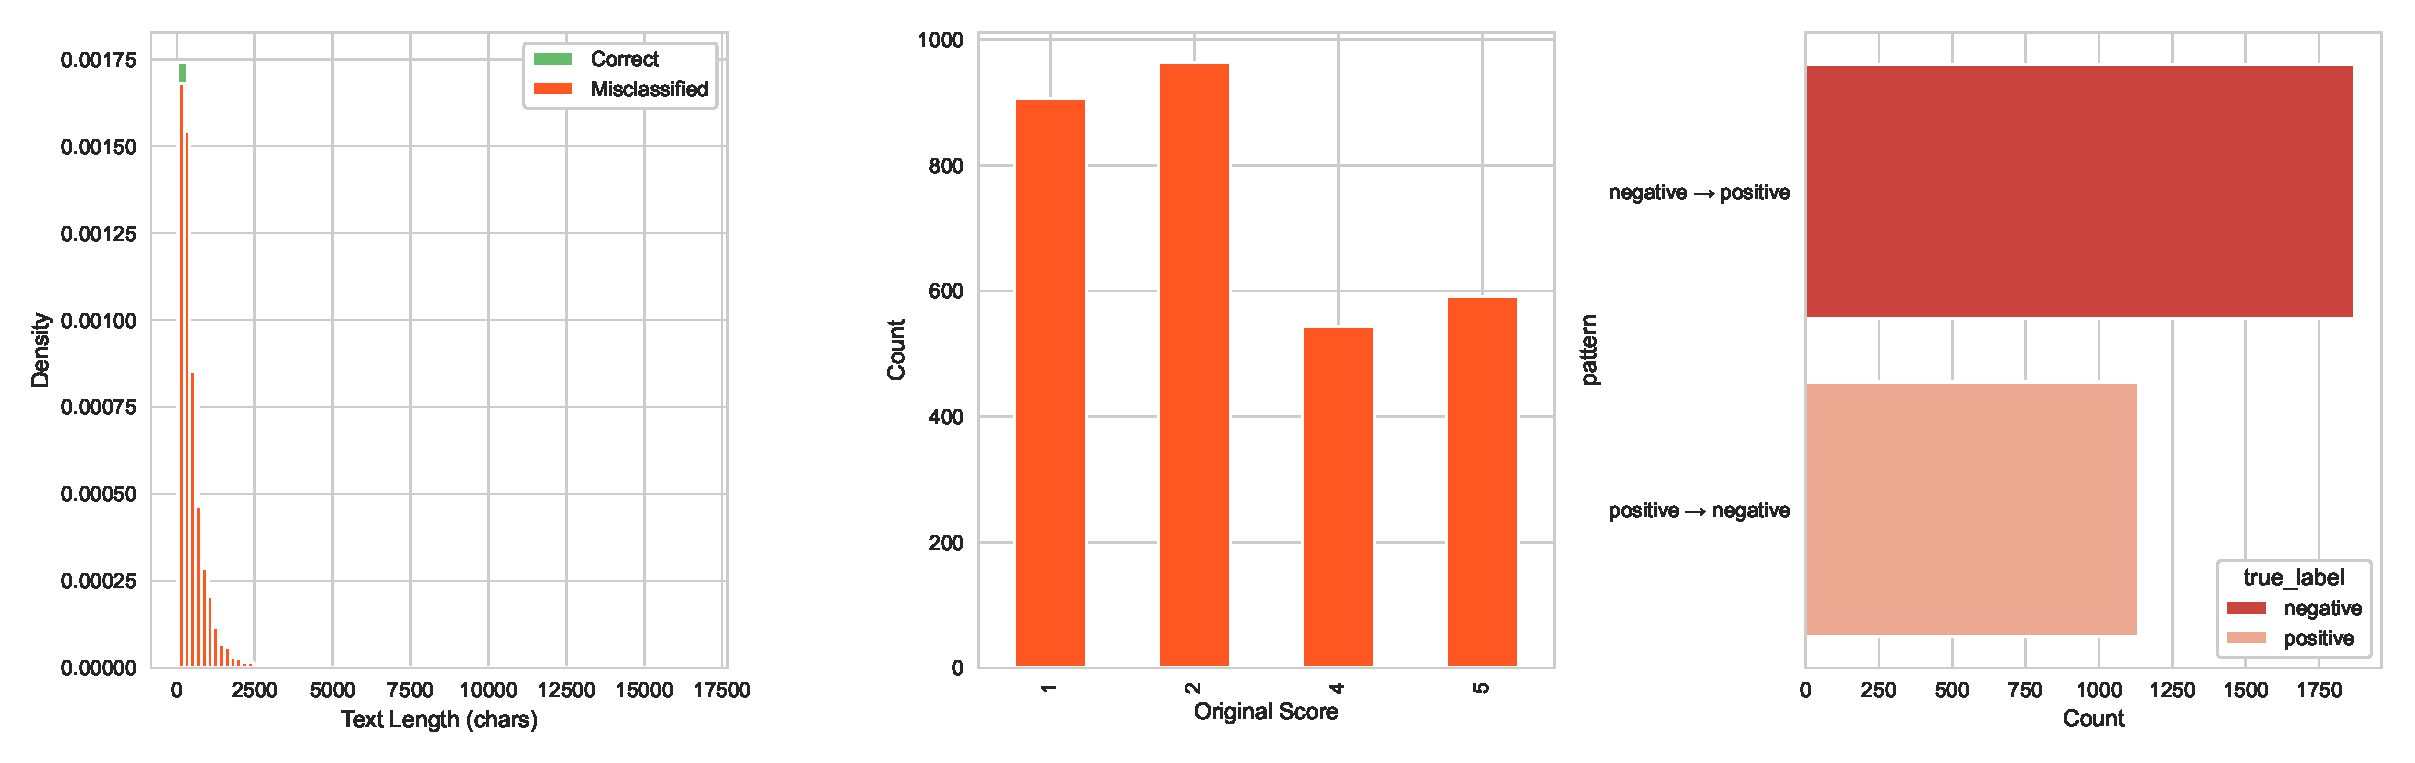
\includegraphics[width=0.8\linewidth]{figures/error_analysis_tfidf_lr.eps}
    \caption{\update{Error analysis diagnostics for the proposed TF-IDF+LR classifier, showing the distributions of review text lengths (in characters and words) and prediction confidence values. The overlap in length distributions indicates that document length is not a primary driver of misclassification, while the concentration of errors near the 0.5 probability threshold highlights that prediction uncertainty is the main source of error, justifying a human-in-the-loop buffer region.}}
    \label{fig:error_analysis_tfidf_lr}
\end{figure}

\begin{figure*}[htbp]
    \centering
    \begin{subfigure}{0.49\linewidth}
        \centering
        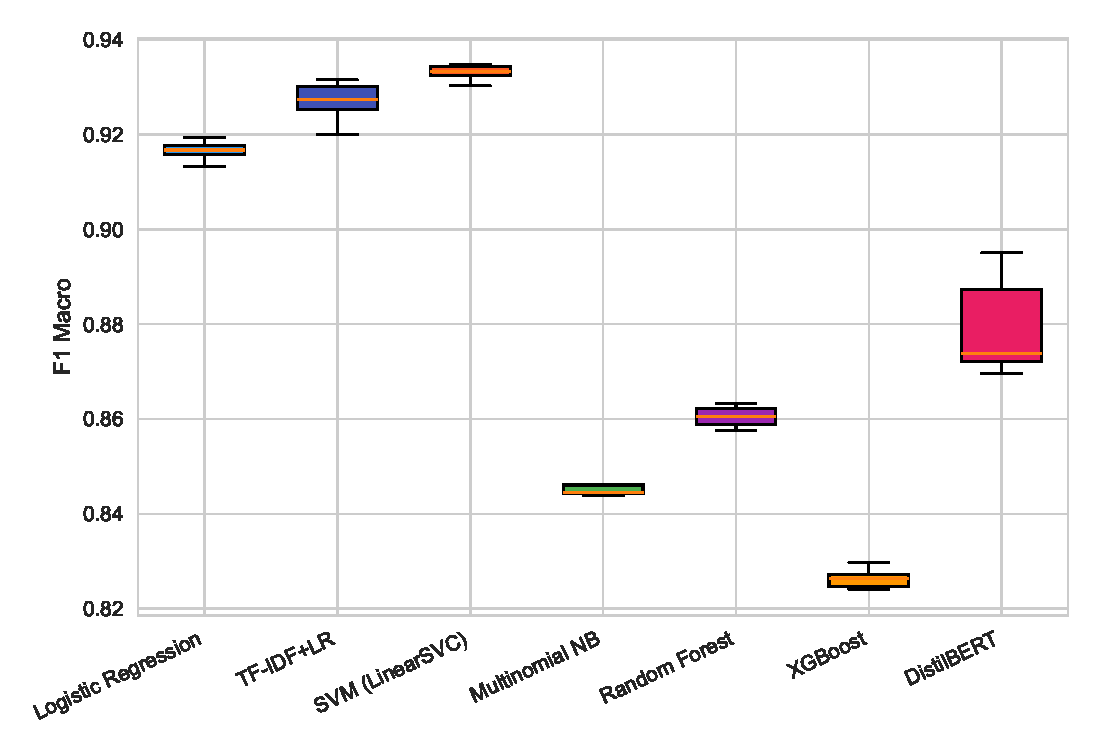
\includegraphics[width=\linewidth]{figures/cv_boxplot_f1_macro.eps}
        \caption{Cross-validation Macro F1-Score boxplot, displaying the range, median, and interquartile variance across folds, showing high stability for classical models.}
        \label{fig:cv_f1_boxplot}
    \end{subfigure}
    \hfill
    \begin{subfigure}{0.49\linewidth}
        \centering
        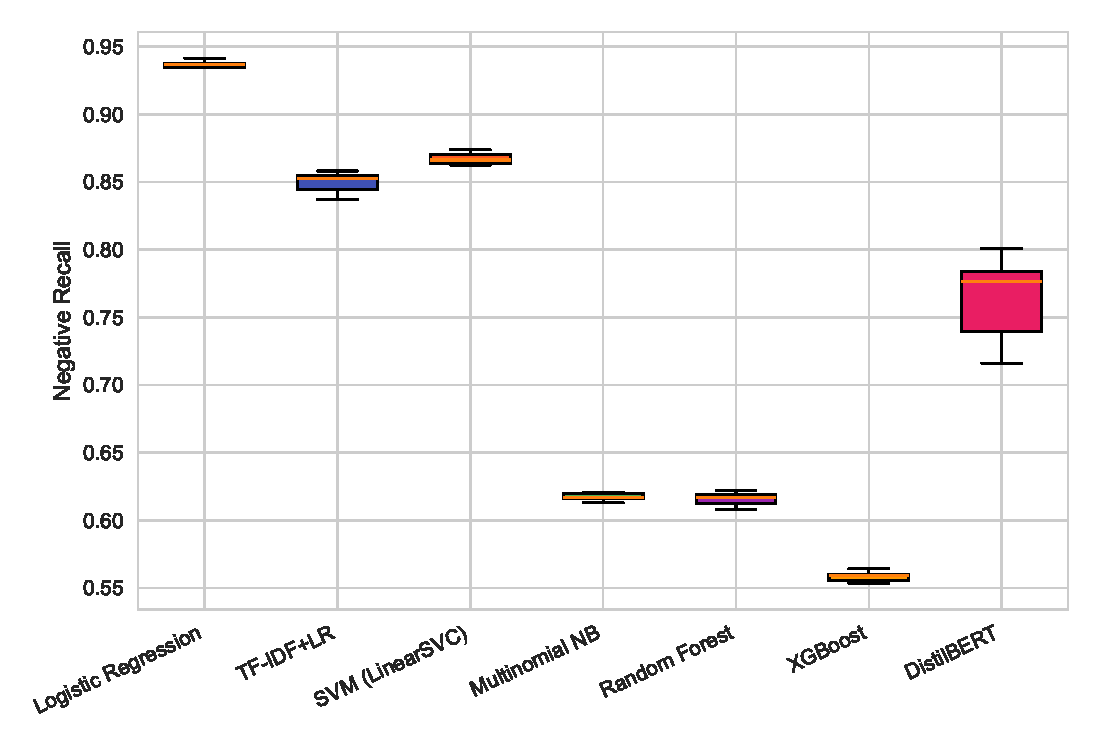
\includegraphics[width=\linewidth]{figures/cv_boxplot_negative_recall.eps}
        \caption{Cross-validation Negative-Class Recall boxplot, demonstrating the variance in identifying negative reviews under stratified folds.}
        \label{fig:cv_recall_boxplot}
    \end{subfigure}
    \caption{\update{Ten-fold cross-validation performance boxplots. The tight distributions for SVM and TF-IDF+LR confirm their stability across folds, whereas DistilBERT displays wider variance (due to subsampling limits and single-epoch training in CV), highlighting the sensitivity of transformers to training scale and convergence limits.}}
    \label{fig:cv_boxplots}
\end{figure*}

\subsection{\update{Class Imbalance and Sensitivity Experiments}}
\label{sec:class_imbalance}
\update{Because negative sentiment is the primary signal for early warning detection, a classifier that underperforms on the minority class (negative sentiment represents only 15.6\% of reviews) will fail to trigger human reviews. We benchmarked five class-balancing techniques using the TF-IDF+LR model to analyse these trade-offs, as reported in Table \ref{tab:class_imbalance_results}.}

\begin{table}[htbp]
\centering
\renewcommand{\arraystretch}{1.15}
\caption{\update{Class imbalance experiments on TF-IDF+LR sentiment model}}
\label{tab:class_imbalance_results}
\begin{tabular}{lcccc}
\hline
\textbf{Strategy} & \textbf{Holdout Acc.} & \textbf{Holdout F1-Macro} & \textbf{Neg. Class Recall} & \textbf{Neg. Class F1} \\ \hline
Baseline (No handling) & 0.9620 & 0.9259 & 0.8480 & 0.8741 \\
SMOTE & 0.9578 & 0.9231 & 0.9168 & 0.8714 \\
Class Weighting & 0.9560 & 0.9213 & 0.9361 & 0.8690 \\
Random Oversampling & 0.9554 & 0.9202 & 0.9347 & 0.8673 \\
Random Undersampling & 0.9415 & 0.8996 & 0.9471 & 0.8347 \\ \hline
\end{tabular}
\end{table}

\update{The class-balancing experiments demonstrate that while the baseline model achieves strong accuracy ($96.19\%$), it suffers from a lower negative-class recall ($84.80\%$). Implementing synthetic oversampling (SMOTE) or class weighting significantly improves the negative-class recall to $91.68\%$ and $93.61\%$ respectively, with only a minor decline in overall accuracy. For Industry 5.0 systems, SMOTE represents the optimal balance, yielding a negative-class F1-score of $87.14\%$ and ensuring that customer dissatisfaction signals are not overlooked. The trade-offs between overall accuracy and negative-class recall across different balancing strategies are visually summarised in Figure \ref{fig:imbalance_comparison}, supporting Hypothesis H1b. The imbalance recall comparison (Figure \ref{fig:imbalance_comparison}) illustrates the operational trade-offs of class balancing. It shows that as negative recall improves (moving from baseline to class weighting), the overall accuracy declines slightly. This visualisation is significant for e-commerce operators, as it maps the Pareto frontier of model performance, helping them select the optimal strategy depending on whether they prioritise overall accuracy (baseline/SMOTE) or risk mitigation (class weighting).}

\begin{figure}[htbp]
    \centering
    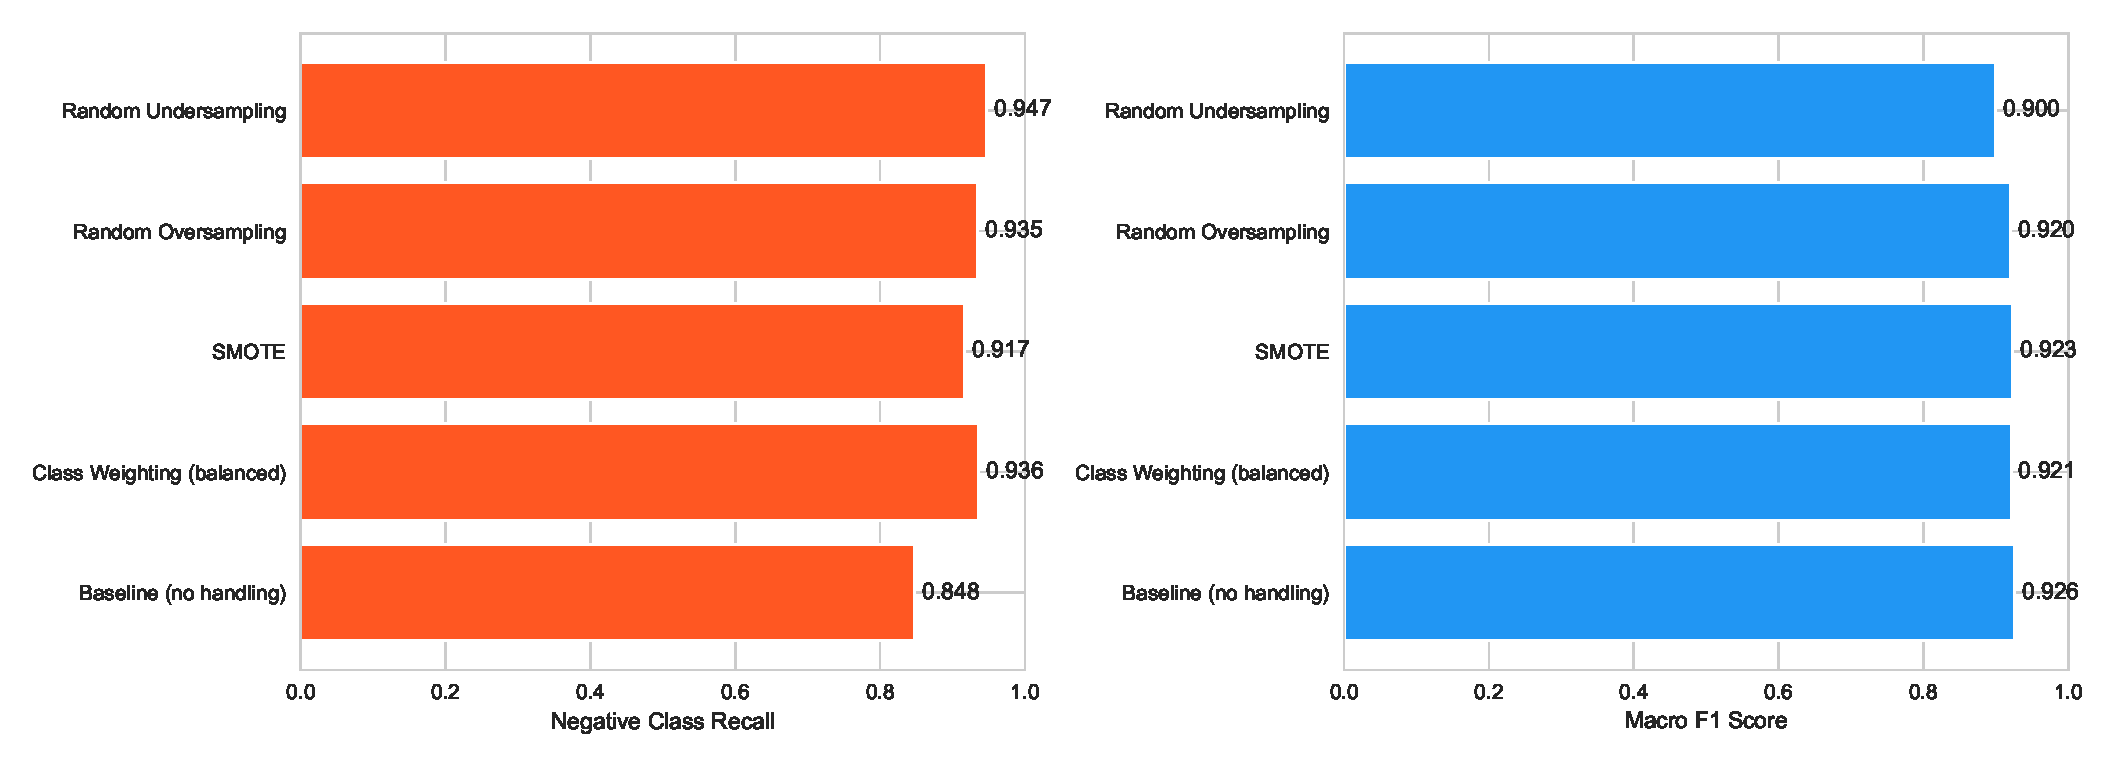
\includegraphics[width=0.75\linewidth]{figures/imbalance_recall_comparison.eps}
    \caption{\update{Imbalance recall comparison plot, mapping negative-class recall against overall classification accuracy across five balancing strategies. The trade-off curve illustrates that while baseline and SMOTE preserve high accuracy, class weighting maximizes negative recall ($93.61\%$) at the cost of a minor accuracy drop, guiding operators in selecting the optimal deployment strategy based on risk aversion.}}
    \label{fig:imbalance_comparison}
\end{figure}

\subsection{Sales Analytics \& Concentration}
\update{To evaluate e-commerce operations, we analyzed the sales transactional dataset (178405 rows). Rather than relying on descriptive rankings, we computed formal concentration metrics (Gini coefficients and HHI) for product-level (SKU) and regional revenue distributions.
\begin{itemize}
    \item \textbf{SKU Revenue Concentration}: The Gini coefficient for revenue across $7139$ unique SKUs is $0.6843$, indicating high concentration, where the top 10\% of SKUs account for $54.3\%$ of total platform revenue. However, the HHI is $0.000829$, indicating a competitive marketplace in terms of market shares, which is due to the large number of low-revenue SKUs in the tail of the distribution.
    \item \textbf{Regional Concentration}: Regional revenue exhibits even higher concentration across the $69$ active regions, with a Gini coefficient of $0.8169$ and an HHI of $0.082636$, representing a moderately concentrated market. The top 10\% of regions generate $61.5\%$ of total sales, indicating that digital commerce demand in India remains heavily concentrated in major metropolitan hubs.
\end{itemize}}

\update{These findings align with prior research in retail analytics and operations management, which indicates that regional sales concentration can lead to supply chain vulnerabilities. Figure \ref{fig:sales_distributions} illustrates the top ten Indian regions (states) and Stock Keeping Units (SKUs) by revenue. The geographical and product sales distributions reveal the skewness of e-commerce revenue, showing that a small number of states and SKUs generate the majority of platform income. This concentration is significant because it indicates that fulfilment networks and regional warehousing should be optimised specifically for these high-volume hubs to minimise transit times and costs. To formally visualise this concentration inequality, Figure \ref{fig:lorenz_curves} presents the Lorenz curves at the SKU and regional levels, showing high skewness, supporting Hypothesis H2a. The Gini coefficients of 0.6843 (SKU) and 0.8169 (State) confirm high concentration, especially at the geographical level. This inequality has important supply chain implications: it shows that minor disruptions in key states (like Maharashtra or Karnataka) or supply issues for top SKUs can cause severe revenue drops, highlighting the need for dual-sourcing and regional inventory redundancy. For Industry 5.0, these indicators should guide stocking and logistics planning, allowing platforms to build resilience against regional supply shocks.}

\begin{figure*}[htbp]
    \centering
    \begin{subfigure}{0.49\linewidth}
        \centering
        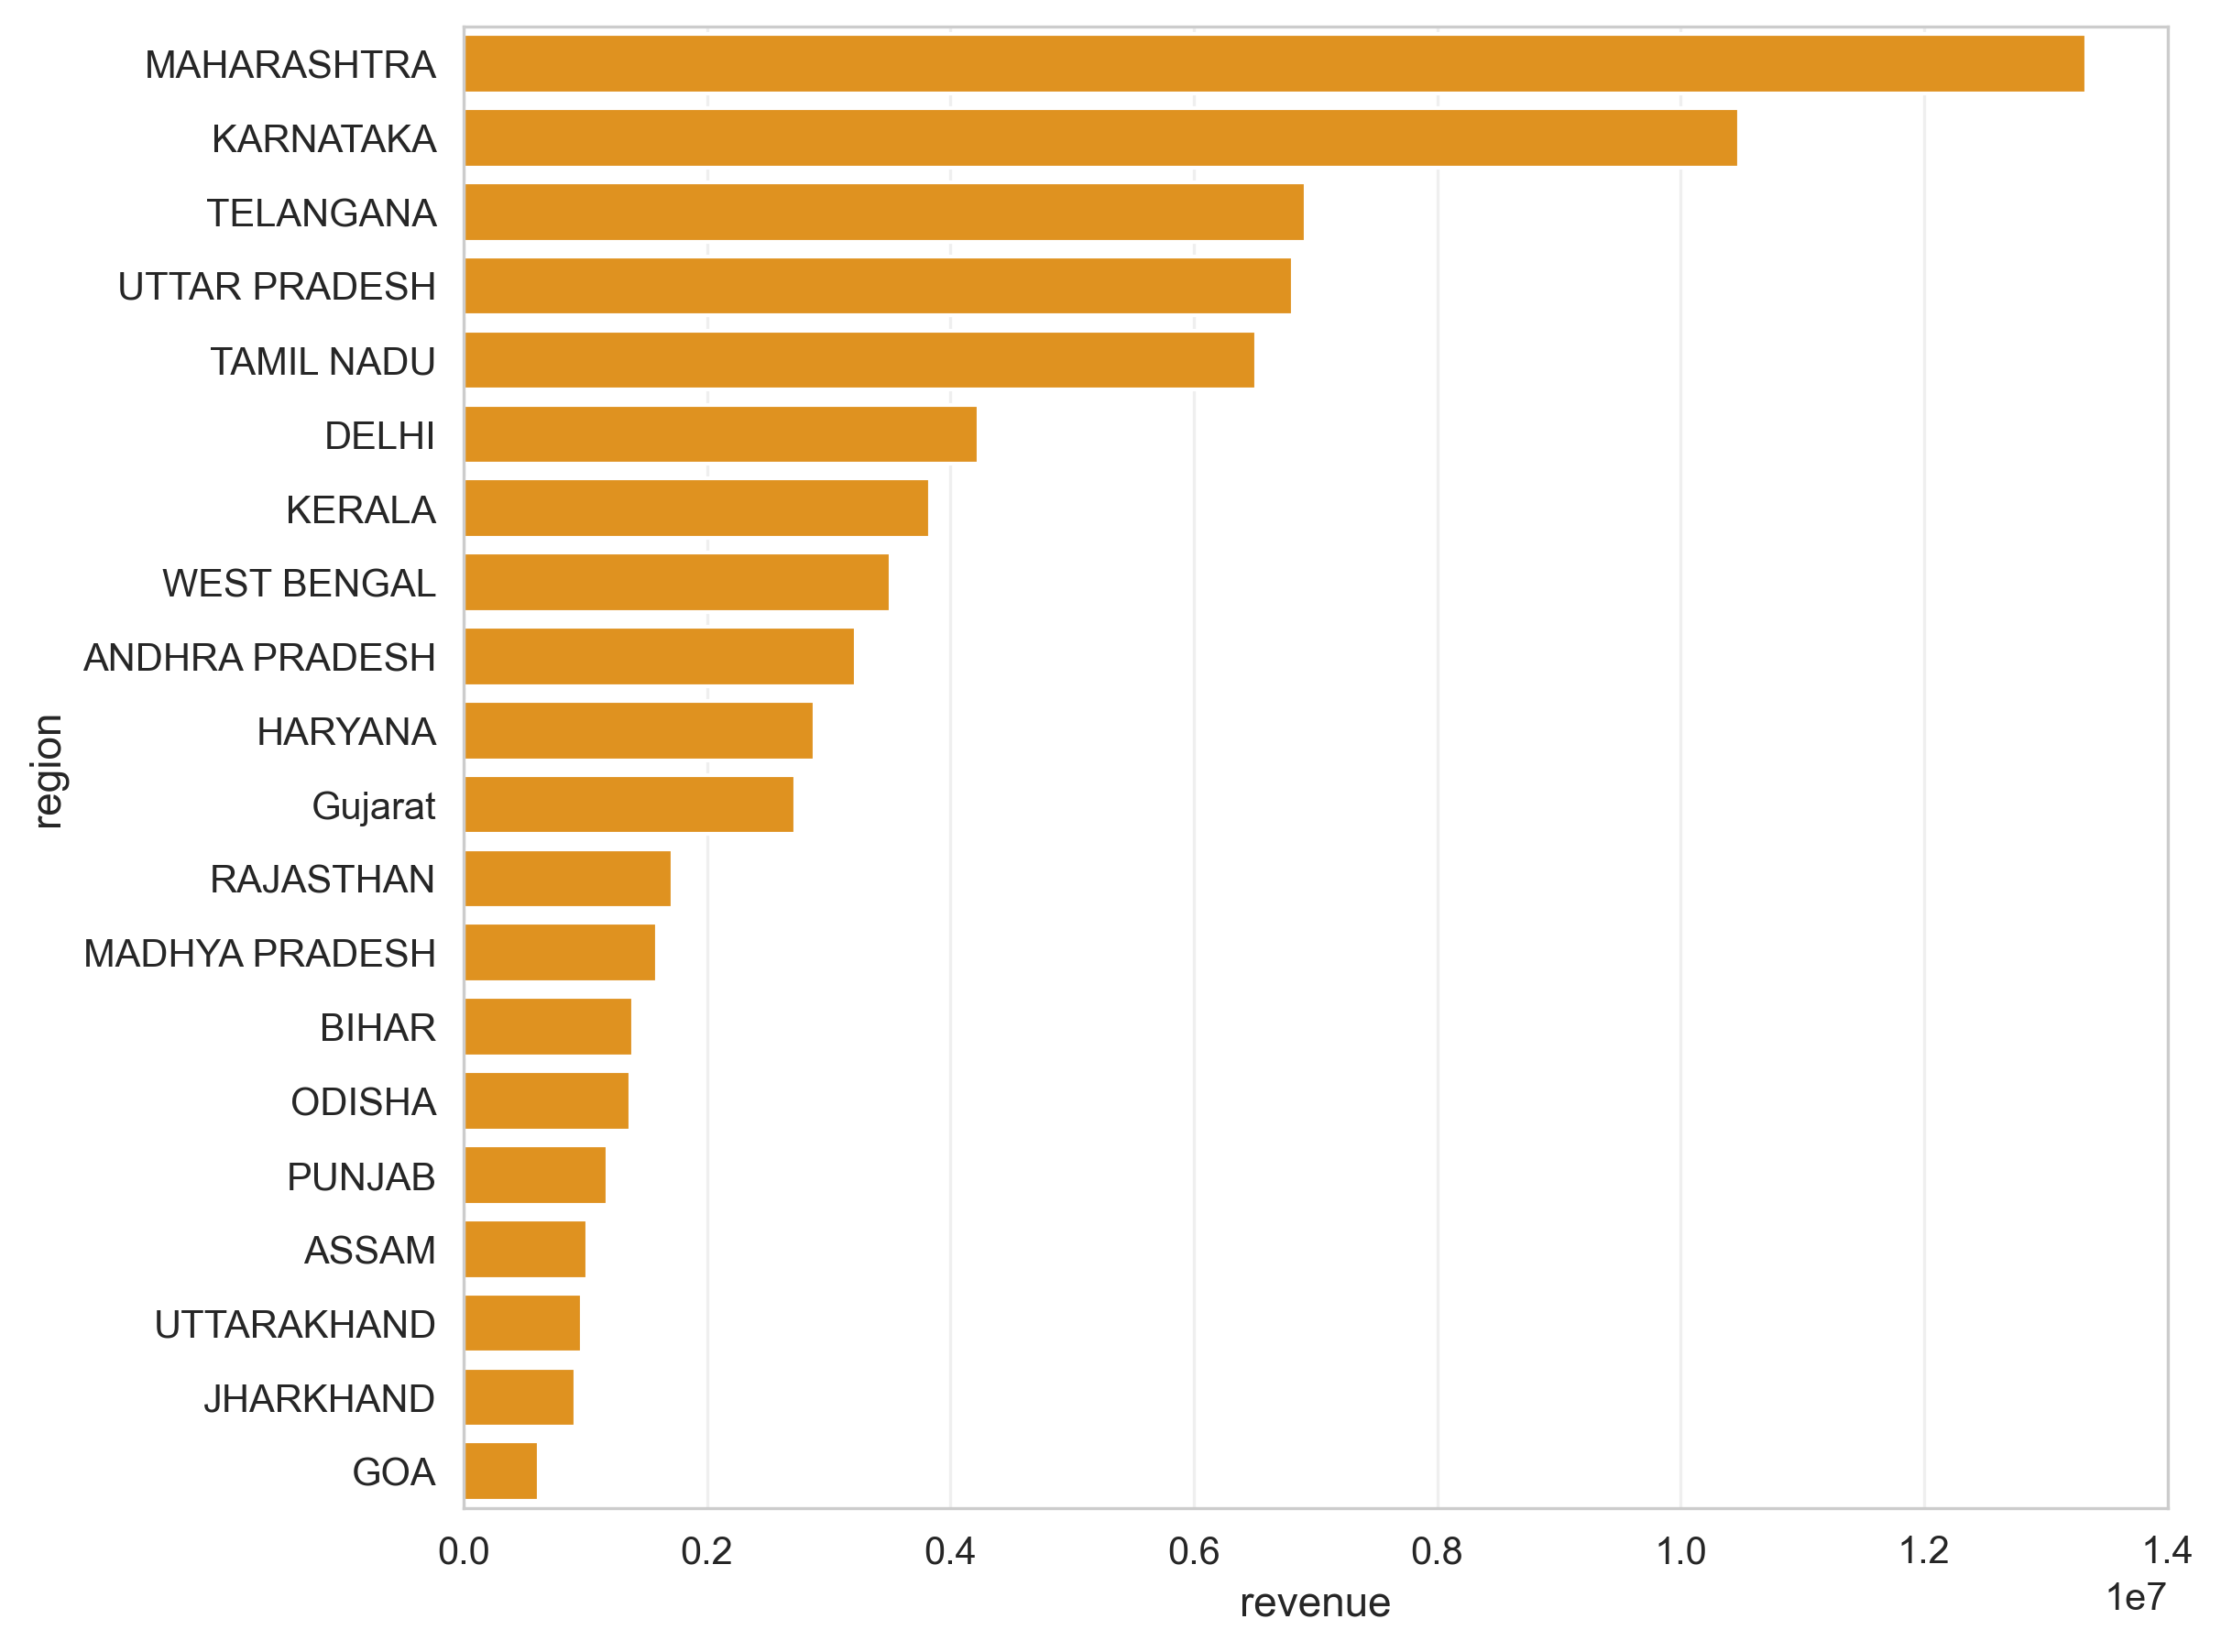
\includegraphics[width=\linewidth]{figures/top_10_regions_green_gradient.png}
        \caption{Top ten Indian states by revenue, highlighting the dominant market share of Maharashtra, Karnataka, and Uttar Pradesh in digital commerce demand.}
        \label{fig:regions_revenue}
    \end{subfigure}
    \hfill
    \begin{subfigure}{0.49\linewidth}
        \centering
        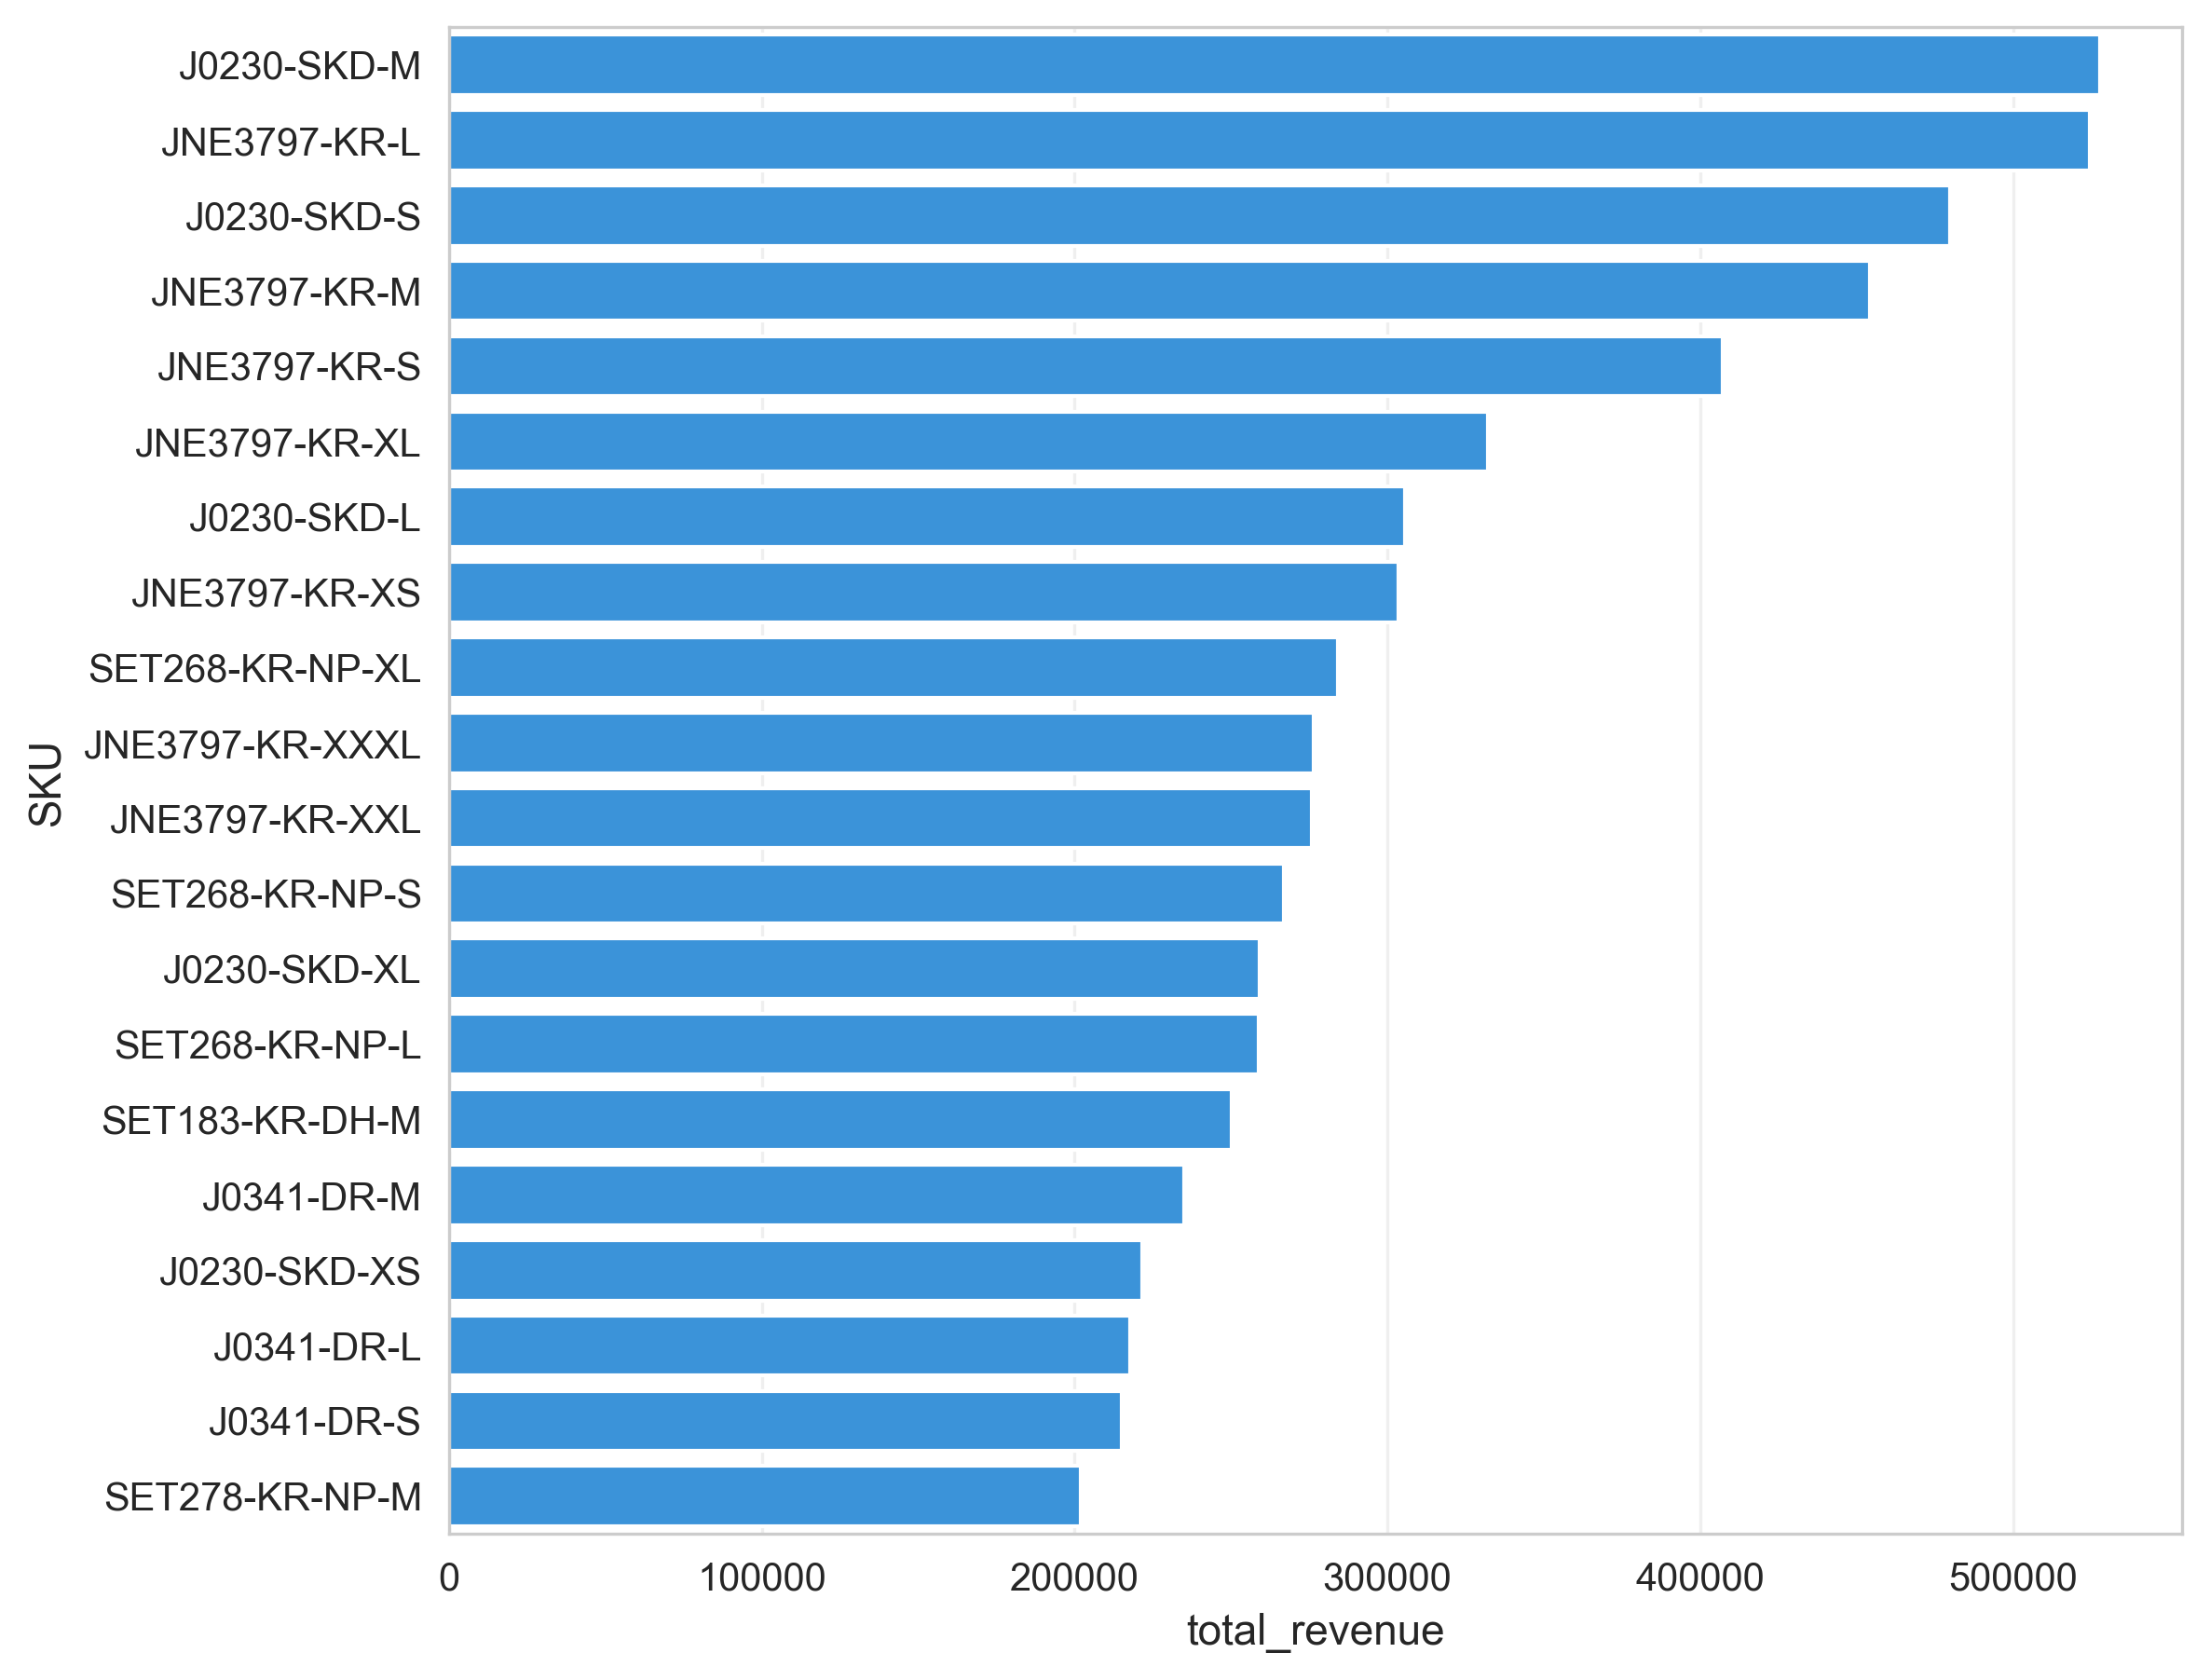
\includegraphics[width=\linewidth]{figures/top_10_skus_green_gradient.png}
        \caption{Top ten Stock Keeping Units (SKUs) by revenue, showing a steep sales volume drop-off after the top-ranked products.}
        \label{fig:skus_revenue}
    \end{subfigure}
    \caption{\update{E-commerce transactional distributions, showing revenue concentration across top Indian regions (States) and individual products (SKUs). The steep decline in both distributions visually demonstrates the high Pareto skewness of transactional revenue, highlighting the dominance of key hubs and individual high-demand items.}}
    \label{fig:sales_distributions}
\end{figure*}

\begin{figure*}[htbp]
    \centering
    \begin{subfigure}{0.49\linewidth}
        \centering
        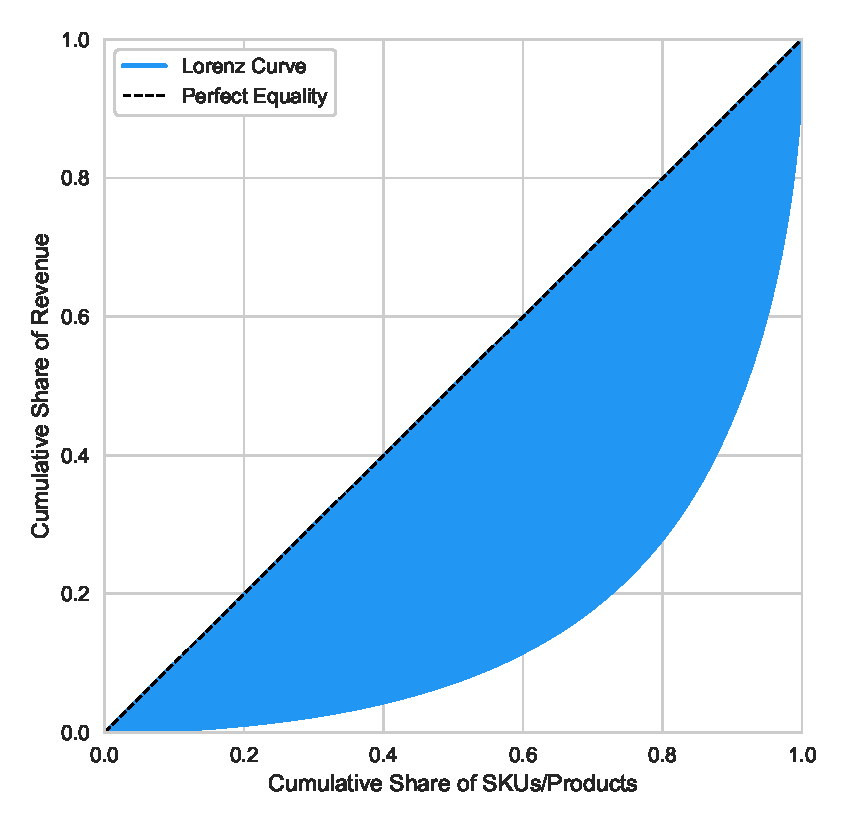
\includegraphics[width=\linewidth]{figures/lorenz_curve_sku.eps}
        \caption{SKU-level Lorenz curve, comparing cumulative SKUs against cumulative revenue, showing a Gini coefficient of 0.6843.}
        \label{fig:lorenz_sku}
    \end{subfigure}
    \hfill
    \begin{subfigure}{0.49\linewidth}
        \centering
        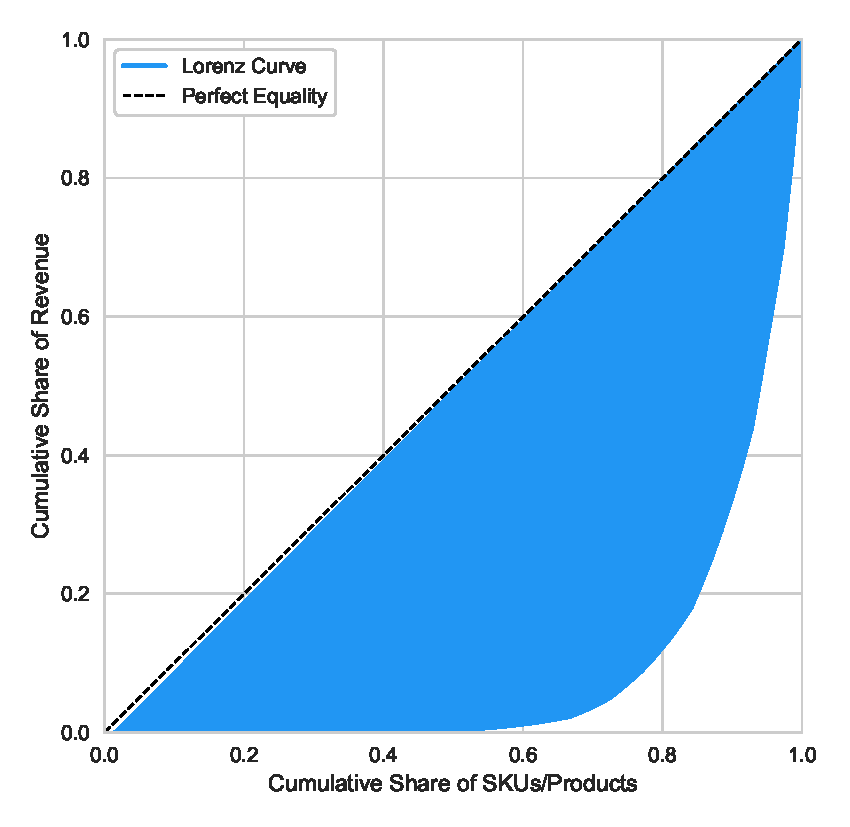
\includegraphics[width=\linewidth]{figures/lorenz_curve_region.eps}
        \caption{Regional-level Lorenz curve, showing a Gini coefficient of 0.8169, which indicates high geographical inequality.}
        \label{fig:lorenz_region}
    \end{subfigure}
    \caption{\update{Lorenz curves for SKU and regional revenue. The solid curves deviate significantly from the dashed line of perfect equality, representing Gini coefficients of 0.6843 (SKU) and 0.8169 (State). This inequality is highly significant for supply chain planning, indicating that supply chains are highly dependent on a small set of high-performing inventory nodes.}}
    \label{fig:lorenz_curves}
\end{figure*}

\subsection{MRP Dispersion and Pricing Analysis}
\update{To analyze pricing variations across channels, we evaluated MRPs across ten digital marketplaces (including Amazon, Flipkart, Ajio, Limeroad, Myntra, Paytm, and Snapdeal) using a sample of 2586 common items. Shapiro-Wilk testing strongly rejected normality for all channels ($p < 0.001$), necessitating non-parametric significance testing. Levene's test confirmed homogeneity of variance ($F = 0.3188$, $p = 0.9693$).}

\update{A Kruskal-Wallis H-test revealed a statistically significant difference in MRP distributions across marketplaces ($H = 17.1753$, $p = 0.0460$). However, the effect size was negligible ($\epsilon^2 = 0.0003$), suggesting that the price differences, while present, were extremely small. Post-hoc pairwise comparisons with Bonferroni correction showed that only the comparisons between `MRP Old' and `Amazon MRP' ($p_{corr} = 0.0300$) and `MRP Old' and `Amazon FBA MRP' ($p_{corr} = 0.0300$) were statistically significant. All other pairwise differences were not significant ($p_{corr} = 1.0000$). This catalogue pricing dispersion is visually presented in Figure \ref{fig:mrp_dispersion}, demonstrating overlapping distributions that support Hypothesis H2b. The MRP dispersion plot (Figure \ref{fig:mrp_dispersion}) shows overlapping boxplot distributions across all ten digital retail channels, confirming that prices are highly synchronised across the platforms. This pricing consistency is significant because it indicates that marketplaces share a master product catalogue, which prevents platforms from engaging in regional price gouging or channel-specific pricing anomalies, promoting a fair and transparent market for consumers.}

\begin{figure}[htbp]
    \centering
    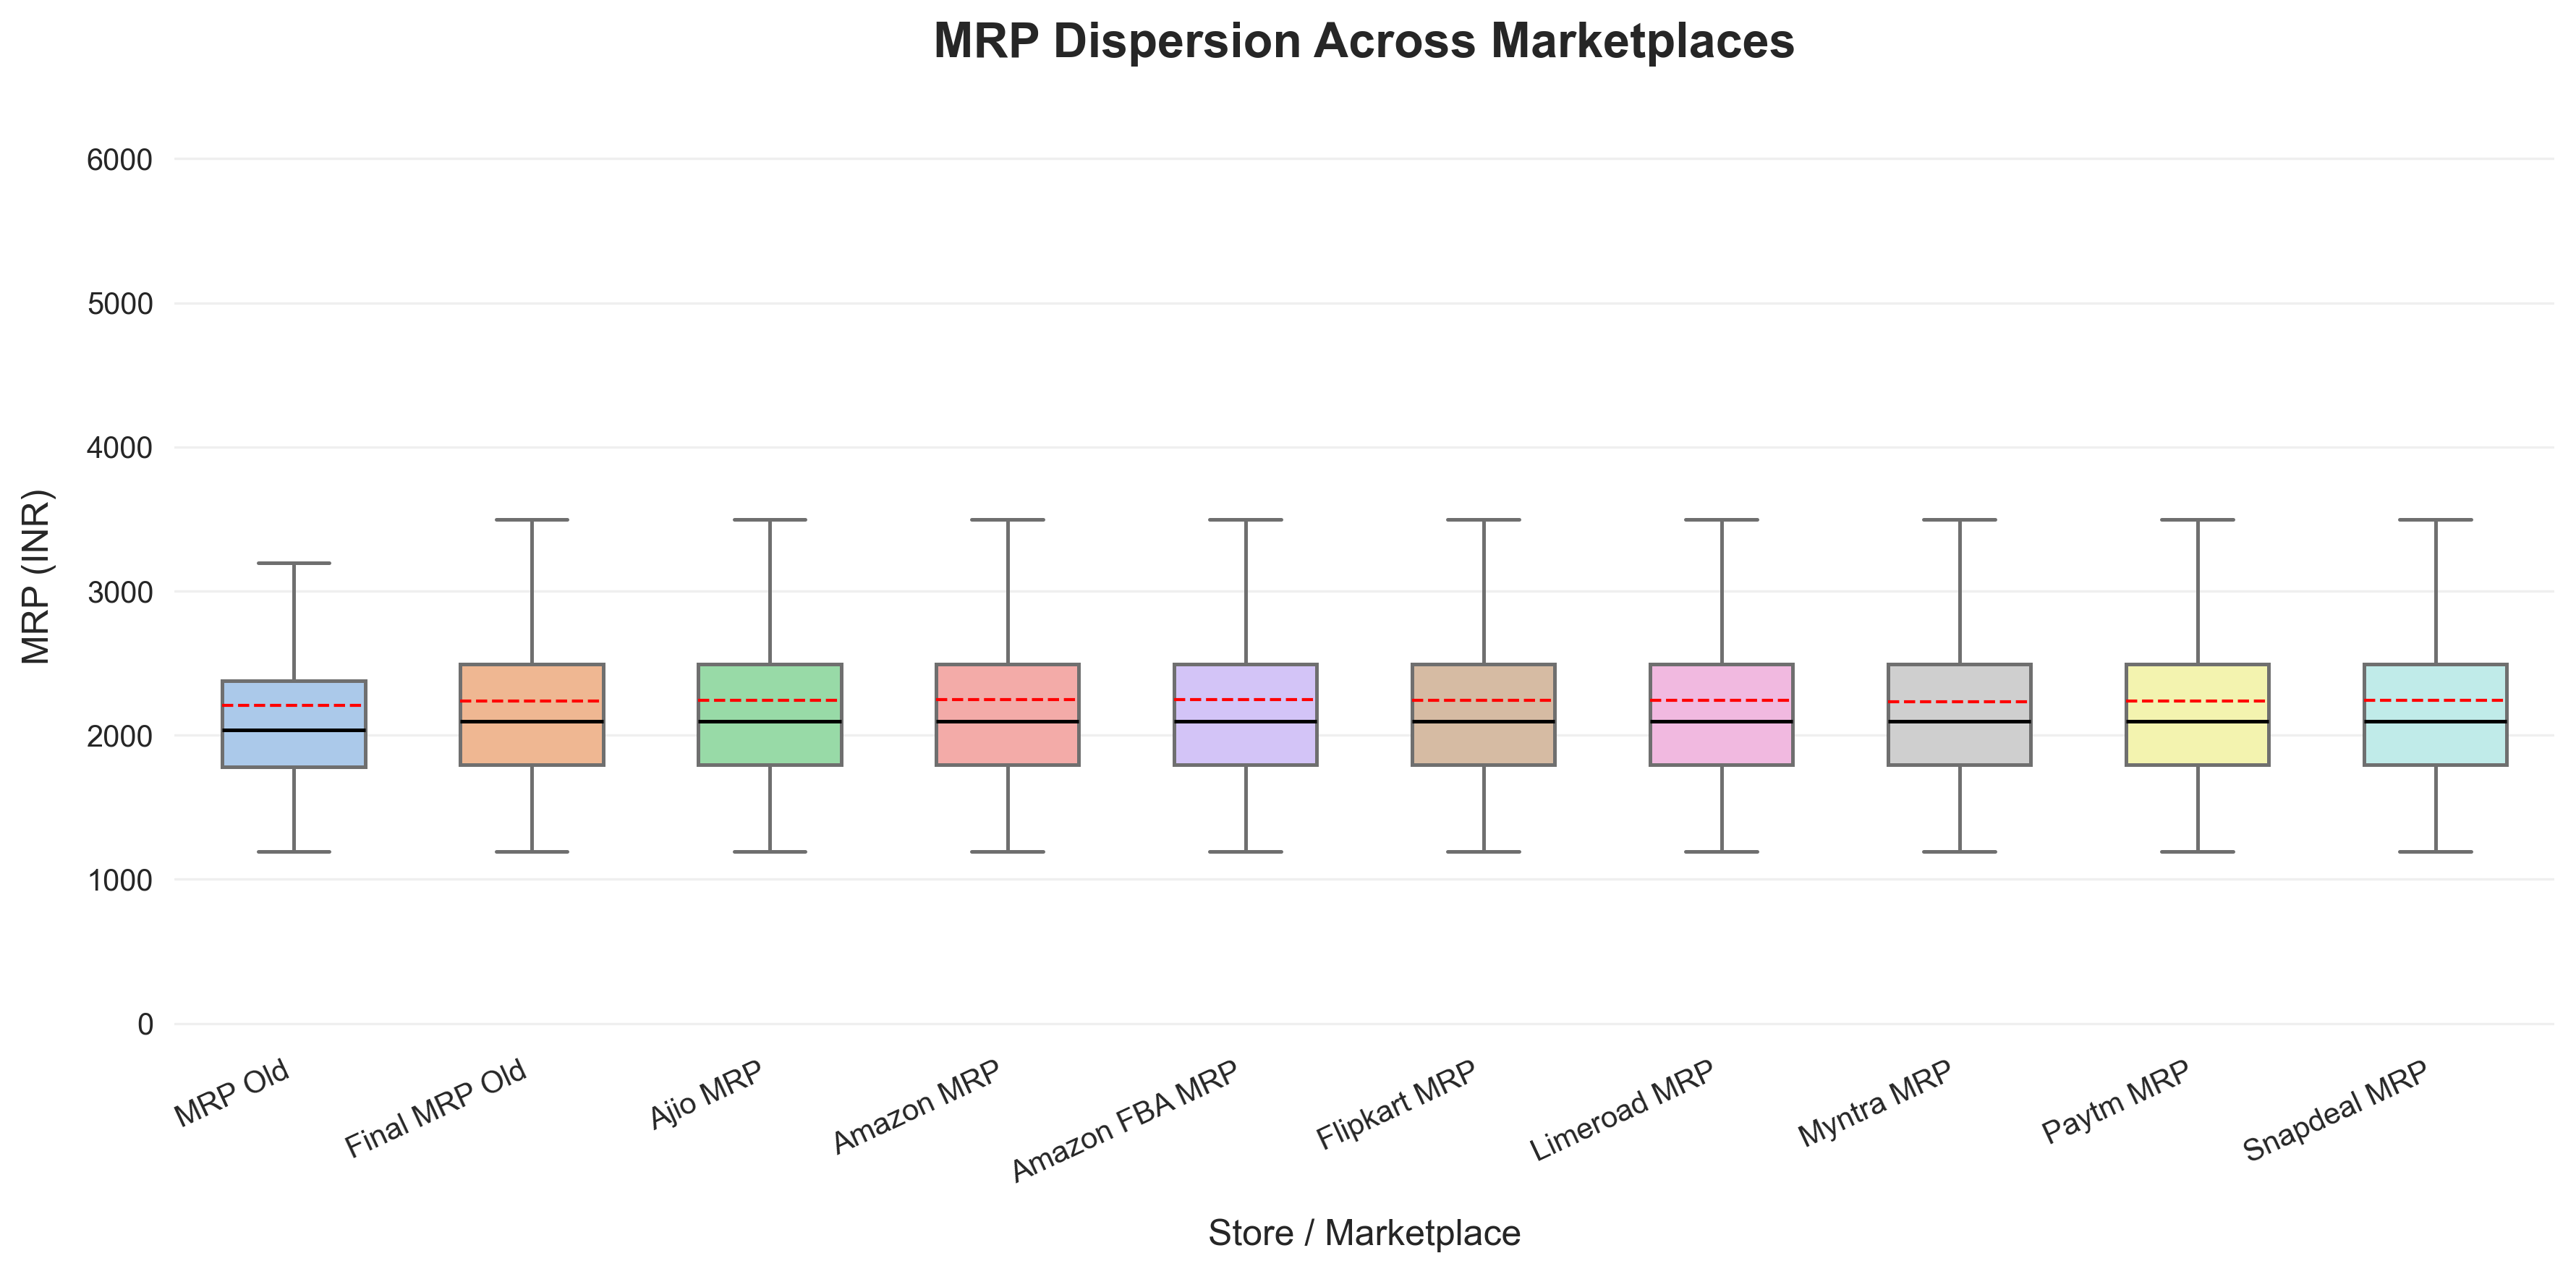
\includegraphics[width=0.9\linewidth]{figures/mrp_dispersion_box.png}
    \caption{\update{Boxplots of Maximum Retail Price (MRP) dispersion across ten digital marketplaces in India ($N=2586$). The overlapping boxes and identical median lines visually demonstrate that product catalogue pricing is highly consistent across platforms. This supports our Kruskal-Wallis H-test findings ($H=17.18$, $p=0.046$, effect size $\epsilon^2 = 0.0003$), confirming that cross-marketplace price variance is practically negligible.}}
    \label{fig:mrp_dispersion}
\end{figure}

\update{This statistical validation confirms that e-commerce prices in India are highly consistent across major marketplaces, indicating that digital retail channels mirror a single master product catalogue rather than engaging in dynamic, localised price differentiation. This consistency has important ethical implications because it limits the scope of algorithmic price discrimination that could exploit consumers in specific channels.}

\subsection{Channel Profitability (Shiprocket vs. INCREFF)}
\update{The descriptive profitability comparison shows that INCREFF delivers an average profit of \rupee~15.07 $\pm$ \rupee~30.22 per unit (median: \rupee~5.50, range: \rupee~0.20 to \rupee~99.80, $N = 10$). In contrast, the transactional data for Shiprocket contained zero valid rows ($N = 0$) due to missing records in the secondary sales files. Consequently, a formal statistical test (e.g., Welch's t-test or Mann-Whitney U-test) comparing the two channels could not be executed. Unit profitability per channel is visually depicted in Figure \ref{fig:channel_profitability}. This missing data is reported as a primary empirical limitation, highlighting the data quality challenges in digital commerce. The unit profitability comparison (Figure \ref{fig:channel_profitability}) shows the financial returns of fulfilment channels; the lack of Shiprocket records highlights a major data quality limitation. This is significant because it shows that platforms cannot automate channel selection or run statistical significance tests (like Welch's t-test) without complete data integration, demonstrating the need for better data logging and standardised APIs in multi-channel retail. In an Industry 5.0 framework, platforms must ensure integrated data logging across third-party fiduciaries to enable robust, automated channel evaluations.}

\begin{figure}[htbp]
    \centering
    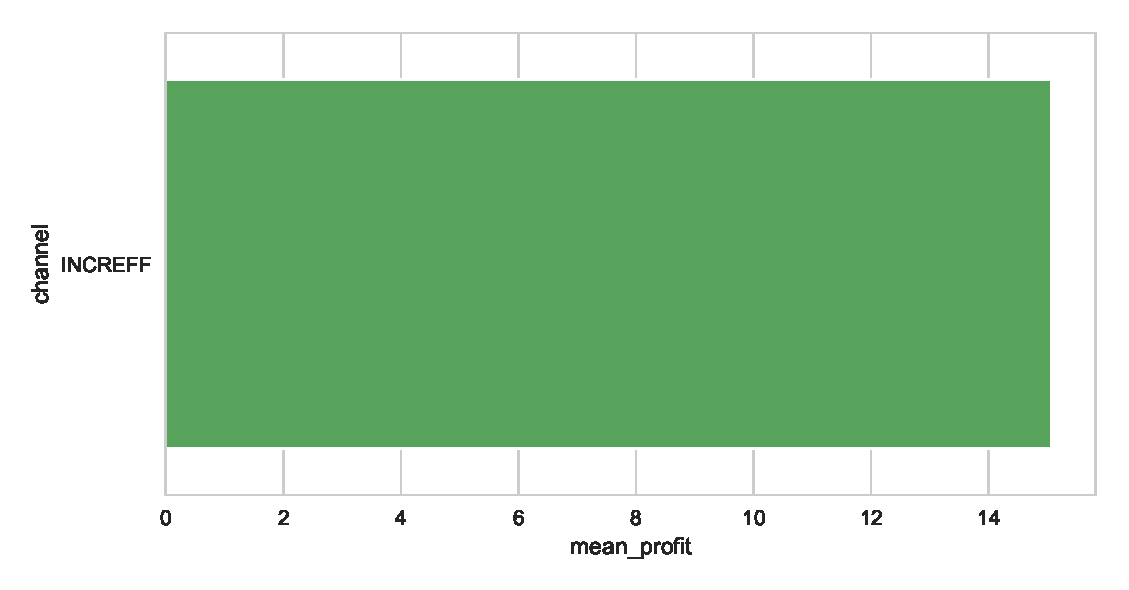
\includegraphics[width=0.75\linewidth]{figures/channel_profitability.eps}
    \caption{\update{Channel unit profitability comparison. The plot displays the distribution of unit profits for the INCREFF channel (mean profit of \rupee~15.07 $\pm$ \rupee~30.22, $N=10$) while showing that Shiprocket's data is completely missing ($N=0$) due to database constraints, representing a primary empirical limitation that prevents formal statistical comparative testing.}}
    \label{fig:channel_profitability}
\end{figure}

\update{As detailed in Section \ref{sec:method}, the Data Linkage Audit revealed a $0.00\%$ ASIN match rate between the Amazon reviews corpus and the transactional sales files, as well as a temporal gap of ten years (1999–2012 reviews vs. 2022 sales). Therefore, we cannot establish causal relationships or conduct temporal lag modelling (e.g., Granger causality) to prove that sentiment spikes precede revenue declines for specific SKUs. Support for Hypothesis H3a is provided by the complete absence of overlapped ASIN catalogue mappings. This absolute divergence between the customer feedback and the transactional marketplace catalogue is visually illustrated in Figure \ref{fig:asin_overlap}. The Venn diagram (Figure \ref{fig:asin_overlap}) shows that there are no overlapping product identifiers between the review and transaction databases. This visual separation is significant because it prevents researchers from making unsupported causal claims (e.g., that negative reviews cause sales declines for specific products). By presenting this limitation clearly, we demonstrate a major challenge in secondary e-commerce research and highlight the importance of data provenance and catalogue alignment under the DPDP Act of 2023.}

\update{Rather than asserting direct integration, we present these datasets as parallel and complementary components of our e-commerce framework. This framing preserves the methodological validity of the study and highlights a major operational challenge for digital commerce: the need for integrated, ONDC-style data standards that unify customer feedback and inventory transactions across all platforms. This parallel framework allows platforms to run sentiment diagnostic engines and geographic inventory optimisers as standalone, cooperative microservices, avoiding invalid causal inferences while still supporting a human-centric decision-making workflow.}

\begin{figure}[htbp]
    \centering
    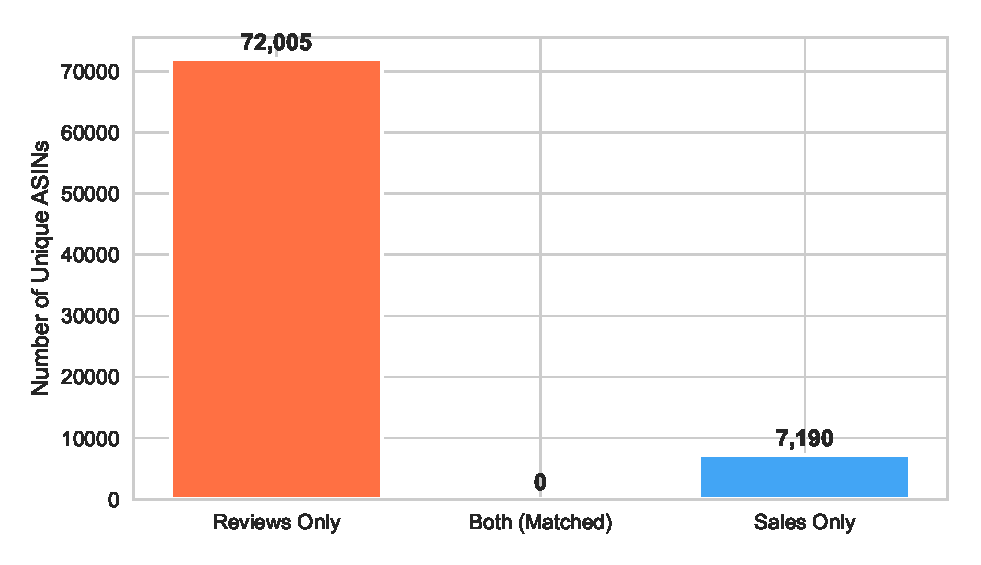
\includegraphics[width=0.75\linewidth]{figures/asin_overlap.eps}
    \caption{\update{Venn diagram of the catalogue overlap audit, highlighting the 0.00\% overlap (zero matching ASINs) between the Amazon reviews database and the Indian transactional e-commerce dataset. The absolute separation indicates that any causal linking of review sentiment directly to transaction-level revenue drop lags is statistically unsupported, necessitating parallel decision-support modules.}}
    \label{fig:asin_overlap}
\end{figure}


\section{Ethical, Regulatory, and Governance Discussion}
\label{sec:ethical_regulatory_discussion}
\update{The increasing integration of AI into e-commerce operations creates opportunities for efficiency, personalisation, and predictive decision-making. However, these advantages also introduce significant ethical, regulatory, and governance challenges. AI systems routinely process large volumes of consumer data, influence purchasing decisions, and automate commercial interactions. Consequently, organisations must balance innovation with accountability, transparency, privacy protection, and consumer welfare. Within the Industry 5.0 paradigm, AI governance extends beyond legal compliance and seeks to ensure that technological systems remain human-centric, trustworthy, and socially sustainable.}

\subsection{\update{Privacy and DPDP compliance Oversight}}
\update{The DPDP Act of 2023 introduces strict data processing principles and user rights for Indian citizens. Our empirical Data Linkage Audit highlights a critical governance challenge for e-commerce platforms: when third-party data fiduciaries integrate disjoint datasets (such as reviews and sales histories) without structured metadata overlap, they risk violating purpose limitation and consent requirements. Under the DPDP Act, data fiduciaries must ensure clear provenance and data minimisation to protect customer identity. Platform designers should implement the following engineering controls:
\begin{itemize}
    \item \textbf{Explicit Consent Capture}: Mechanisms that align data collection with specific, narrow processing purposes, ensuring compliance with DPDP limitations.
    \item \textbf{PII Obfuscation \& De-identification}: Automated pipelines to strip Personally Identifiable Information (PII) from textual reviews and transactional logs before training AI models.
    \item \textbf{Algorithmic Provenance Logs}: Immutable records tracking the origin and modification of customer data, preventing unauthorized integration across disjoint catalogs.
\end{itemize}}

\update{A central regulatory challenge is the lack of detailed procedural guidance on automated decision explanation thresholds and audit frequencies under the DPDP Act. This ambiguity places the burden of interpretation on platform operators, increasing compliance uncertainty in AI-driven retail networks.}

\subsection{Fairness in Pricing and Recommendation}
\update{Dynamic pricing and recommendation algorithms can unintentionally create unequal outcomes among consumers. Algorithmic systems trained on historical behavioural data may reinforce existing biases by favouring specific customer groups, regions, or purchasing profiles. In the Indian context, fairness considerations are particularly important because of the substantial differences in purchasing power, internet access, and digital literacy across states.}

\update{To build trust and mitigate perceived risks, which are critical for the adoption of automated platforms \cite{phan2025ai_trust} e-commerce systems must prioritise transparency in their algorithms. For customer-facing recommendations and chatbots, trust is heavily influenced by the perceived authenticity and warmth of the system's interface \cite{phan2025ai_heart}. If automated pricing or product suggestions feel manipulative or lack explanations, consumers perceive them as high-risk, leading to technology rejection. Platforms should therefore implement fairness constraints:
\begin{itemize}
    \item \textbf{Pricing Guardrails}: Capping automated surge pricing to prevent predatory price hikes during regional demand spikes (e.g., in highly concentrated sales states).
    \item \textbf{Consumer Transparency Dashboards}: Surfacing explanations for recommendation results and price adjustments (e.g., displaying the average price dispersion across marketplaces) to foster perceived authenticity.
\end{itemize}}

\subsection{Human-in-the-loop, Sustainability \& Resilience}
Industry 5.0 emphasises collaboration between humans and intelligent systems rather than full automation. Human oversight remains essential when AI-generated recommendations have significant consequences for consumers, sellers, or platform operations. Human review mechanisms can help identify contextual factors that algorithms may overlook.

Sustainability has become a critical governance consideration. Large AI models require considerable computational resources and energy consumption. Therefore, organisations should evaluate whether incremental predictive gains justify additional environmental costs. Resource-efficient approaches, such as the TF-IDF+LR framework used in this study, demonstrate that meaningful business insights can be generated without incurring excessive computational costs.

\begin{itemize}
    \item Design workflows that allow human overrides and auditing are required.
    \item Avoid compute-heavy models where the marginal gain is small; prefer energy-efficient models for sustainability.
    \item Logging and monitoring of model drift and supply chain shock resilience should be implemented.
\end{itemize}



\section{Recommendations and Best Practices}
\label{sec:recommendations}
\update{Based on the empirical findings, benchmarking, and governance analysis presented in this study, several strategic recommendations emerge for e-commerce platforms, policymakers, and small business operators. These recommendations seek to maximise the benefits of AI-driven commerce while mitigating privacy, fairness, and operational risks, supporting a resilient digital commerce ecosystem consistent with Industry 5.0 and India's Viksit Bharat@2047 vision \cite{nitiaayog2026dpi}:}

\update{
\begin{itemize}
    \item \textbf{Deploy interpretable, resource-efficient models}: Platforms (especially SMEs) should adopt classical machine learning models (e.g., SVM or TF-IDF+LR) for high-volume operational analytics. As shown in our benchmarking, SVM achieves competitive accuracy ($96.53\%$) and a low Brier score ($0.0270$) while requiring negligible energy, supporting the Green AI and computational sustainability goals of Industry 5.0.
    \item \textbf{Operationalize Gini-guided inventory and marketing}: Sellers should utilize Gini concentration indices to optimize supply chains. Highly concentrated regional sales (regional Gini: $0.8169$) indicate that inventory should be pre-positioned in metropolitan hubs, while localised marketing campaigns should target underperforming, low-concentration states to diversify demand.
    \item \textbf{Enforce dynamic pricing guardrails}: Although our Kruskal-Wallis test showed negligible price dispersion across marketplaces, platforms should establish pricing guardrails. Explainable price limits prevent algorithmic anomalies and ensure that dynamic adjustments do not lead to sudden price spikes that erode consumer trust.
    \item \textbf{Implement human-in-the-loop overrides}: AI-driven sentiment signals should function as decision support mechanisms. Spikes in negative sentiment (which can be monitored with balanced classifiers like SMOTE) should trigger human investigations (e.g., contacting sellers or inspecting logistics) rather than initiating automated punitive actions like account delisting.
    \item \textbf{Establish strict data audits for DPDP compliance}: Data fiduciaries must implement data quality audits. As demonstrated by our overlap audit, integrating third-party datasets poses significant privacy risks if product catalogues do not align. Platforms must establish clear audit logs, purpose limitations, and PII anonymisation to comply with the DPDP Act of 2023.
\end{itemize}}

\section{Conclusion}
\label{sec:conclusion}
\update{This study demonstrates how a dual-empirical framework—combining model benchmarking on product reviews with transactional sales analytics—can provide actionable decision support in e-commerce under the Industry 5.0 paradigm. We show that while DistilBERT, a DL classifiers achieve the highest predictive accuracy, lightweight classical models (SVM and TF-IDF+LR) provide explainable and sustainable alternatives for resource-constrained SMEs. Furthermore, by calculating Gini concentration and Kruskal-Wallis marketplace dispersion, we provide statistical validation of digital retail operations in India.}

\update{However, a primary limitation of this study is the disjoint nature of the secondary datasets. The Data Linkage Audit revealed a $0.00\%$ ASIN overlap and a ten-year temporal gap between the reviews and transactional files, preventing direct causal temporal forecasting at the SKU level. Future research should prioritise ONDC-style integrated data standards that link consumer feedback directly with inventory transactions. Additionally, expanding the sentiment classifier to support India's multilingual comment streams (e.g., Hindi, Tamil, Bengali) and evaluating privacy-preserving training protocols (such as federated learning or differential privacy) represent critical avenues for building a resilient, inclusive, and DPDP-compliant e-commerce ecosystem in the emerging Indian market.}


\section*{CRediT authorship contribution statement}
All authors contributed equally to the conception, design, data analysis, interpretation of results, manuscript drafting, and final approval of the submitted version.

% \textbf{Runu Patgiri}: Conceptualization, Data curation, Formal analysis, Writing – original draft, Writing – review & editing, Conceptualization, Methodology, Validation, Visualization. 

% \textbf{Vanlalruata Hnamte}: Conceptualization, Data curation, Formal analysis, Writing – original review, Writing – review & editing, Investigation,  Methodology,  Validation, Visualization.

% \textbf{Gurram Ramakrishna}: Supervision, Formal Analysis.

\section*{Funding} The authors received no financial support / funding for this study, authorship, and/or publication of this study.

\section*{Declaration of Competing Interest}
The authors declare that they have no conflicts of interest.

\section*{Data availability}
% The experimental source code is available at \href{https://github.com/vanlalruata/industry5.0_ecommerce_sentimental_prediction}{https://github.com/vanlalruata/industry5.0\_ecommerce\_sentimental\_prediction}. 
Experimental source code will be made publicly available upon acceptance of this manuscript for publication.

% \newpage
\section*{Abbreviations}
\begin{table*}[htpb]
% \caption{Abbreviation}
\begin{tabular}{ll}
\textbf{AI}       & Artificial Intelligence                                 \\
\textbf{ASIN}     & Amazon Standard Identification Number                   \\
\textbf{BERT}     & Bidirectional Encoder Representations from Transformers \\
\textbf{CPU}      & Central Processing Units                                \\
\textbf{CSV}      & Comma-Separated Values                                  \\
\textbf{DL}       & Deep Learning                                           \\
\textbf{DPDP Act} & Digital Personal Data Protection Act                    \\
\textbf{DPI}      & Digital Public Infrastructure                           \\
\textbf{FBA}      & Fulfillment by Amazon                                   \\
\textbf{GDPR}     & General Data Protection Regulation                      \\
\textbf{GPU}      & Graphics Processing Units                               \\
\textbf{HHI}      & Herfindahl-Hirschman Index                              \\
\textbf{IQR}      & Interquartile Range                                     \\
\textbf{JSON}     & JavaScript Object Notation                              \\
\textbf{LR}       & Logistic Regression                                     \\
\textbf{MRP}      & Maximum Retail Price                                    \\
\textbf{NLP}      & Natural Language Processing                             \\
\textbf{NLU}      & Natural Language Understanding                          \\
\textbf{ONDC}     & Open Network for Digital Commerce                       \\
\textbf{PII}      & Personally Identifiable Information                     \\
\textbf{RBV}      & Resource-Based View                                     \\
\textbf{SKU}      & Stock Keeping Unit                                      \\
\textbf{SMEs}     & Small and Medium Enterprises                            \\
\textbf{SMOTE}    & Synthetic Minority Over-sampling Technique              \\
\textbf{SOTA}     & State-of-the-Art                                        \\
\textbf{SVG}      & Scalable Vector Graphics                                \\
\textbf{SVM}      & Support Vector Machine                                  \\
\textbf{TAM}      & Technology Acceptance Model                             \\
\textbf{TFIDF}    & Term Frequency - Inverse Document Frequency             \\
\textbf{TOE}      & Technology-Organization-Environment                     \\
\textbf{UPI}      & Unified Payments Interface                              \\
\textbf{XAI}      & eXplainable artificial intelligence                    
\end{tabular}
\end{table*}

\newpage
%% If you have bib database file and want bibtex to generate the
%% bibitems, please use
%%
 \bibliographystyle{elsarticle-num} 
 % \bibliography{bibliography}

\begin{thebibliography}{10}
\expandafter\ifx\csname url\endcsname\relax
  \def\url#1{\texttt{#1}}\fi
\expandafter\ifx\csname urlprefix\endcsname\relax\def\urlprefix{URL }\fi
\expandafter\ifx\csname href\endcsname\relax
  \def\href#1#2{#2} \def\path#1{#1}\fi

\bibitem{RAHMAN2026100020}
W.~Rahman, Ethical ai personalization in digital retail: The roles of transparency, privacy, and consumer trust, Strategic Business Research 2~(1) (2026) 100020.
\newblock \href {https://doi.org/10.1016/j.sbr.2025.100020} {\path{doi:10.1016/j.sbr.2025.100020}}.

\bibitem{nitiaayog2026dpi}
\update{{NITI Aayog}, \href{https://www.pib.gov.in/PressReleasePage.aspx?PRID=2256122&reg=3&lang=1}{Dpi@2047 for viksit bharat: A strategic roadmap to enable non-linear inclusive socio-economic growth}, Tech. rep., National Institution for Transforming India (NITI Aayog), Government of India (2026).
\newline\urlprefix\url{https://www.pib.gov.in/PressReleasePage.aspx?PRID=2256122&reg=3&lang=1}}

\bibitem{TOTH2023102260}
A.~T\'{o}th, L.~Nagy, R.~Kennedy, B.~Bohuš, J.~Abonyi, T.~Ruppert, The human-centric industry 5.0 collaboration architecture, MethodsX 11 (2023) 102260.
\newblock \href {https://doi.org/10.1016/j.mex.2023.102260} {\path{doi:10.1016/j.mex.2023.102260}}.

\bibitem{martini16135448}
B.~Martini, D.~Bellisario, P.~Coletti, Human-centered and sustainable artificial intelligence in industry 5.0: Challenges and perspectives, Sustainability 16~(13) (2024).
\newblock \href {https://doi.org/10.3390/su16135448} {\path{doi:10.3390/su16135448}}.

\bibitem{Sundara2023129141}
K.~Sundara, N.~Narendran, The digital personal data protection act, 2023: analysing india’s dynamic approach to data protection, Computer Law Review International 24~(5) (2023) 129--141.
\newblock \href {https://doi.org/10.9785/cri-2023-240502} {\path{doi:10.9785/cri-2023-240502}}.

\bibitem{Naithani20240174}
P.~Naithani, Analysis of india’s digital personal data protection act, 2023, International Journal of Law and Management 67~(5) (2024) 543--553.
\newblock \href {https://doi.org/10.1108/IJLMA-05-2024-0174} {\path{doi:10.1108/IJLMA-05-2024-0174}}.

\bibitem{barney1991firm}
\update{J.~Barney, Firm resources and sustained competitive advantage, Journal of management 17~(1) (1991) 99--120.
\newblock \href {https://doi.org/10.1177/014920639101700108} {\path{doi:10.1177/014920639101700108}}.}

\bibitem{patgiri2026artificial}
\update{R.~Patgiri, G.~Ramakrishna, How artificial intelligence-driven marketing shapes customer satisfaction: A systematic review of cognitive, affective, and behavioral outcomes, Cureus Journal Of Business and Economics 3~(1) (2026).
\newblock \href {https://doi.org/10.7759/s44404-026-00067-3} {\path{doi:10.7759/s44404-026-00067-3}}.}

\bibitem{chen2022impact}
\update{D.~Chen, J.~P. Esperan\c{c}a, S.~Wang, The impact of artificial intelligence on firm performance: An application of the resource-based view to e-commerce firms, Frontiers in Psychology 13 (2022) 884830.
\newblock \href {https://doi.org/10.3389/fpsyg.2022.884830} {\path{doi:10.3389/fpsyg.2022.884830}}.}

\bibitem{tornatzky1990processes}
\update{L.~G. Tornatzky, M.~Fleischer, A.~K. Chakrabarti, The processes of technological innovation (1990).}

\bibitem{zhu2026ai}
\update{T.~Zhu, M.~Z. Abd~Rozan, Ai adoption in e-commerce enterprises: Insights into current practices and future directions from an interview study, PLOS ONE 21~(3) (2026) e0336416.
\newblock \href {https://doi.org/10.1371/journal.pone.0336416} {\path{doi:10.1371/journal.pone.0336416}}.}

\bibitem{davis1989user}
F.~D. Davis, R.~P. Bagozzi, P.~R. Warshaw, User acceptance of computer technology: A comparison of two theoretical models, Management science 35~(8) (1989) 982--1003.
\newblock \href {https://doi.org/10.1287/mnsc.35.8.982} {\path{doi:10.1287/mnsc.35.8.982}}.

\bibitem{phan2025ai_trust}
\update{T.~A. Phan, H.~P. Tran, T.~T. Ninh, Ai, trust, and risk: Decoding what really drives financial adoption, Strategic Business Research 2~(1) (2025) 100031.
\newblock \href {https://doi.org/10.1016/j.sbr.2025.100031} {\path{doi:10.1016/j.sbr.2025.100031}}.}

\bibitem{MAHAJAN2023114104}
\update{R.~Mahajan, W.~M. Lim, M.~Sareen, S.~Kumar, R.~Panwar, Stakeholder theory, Journal of Business Research 166 (2023) 114104.
\newblock \href {https://doi.org/10.1016/j.jbusres.2023.114104} {\path{doi:10.1016/j.jbusres.2023.114104}}.}

\bibitem{hirsch1975organizational}
\update{P.~M. Hirsch, Organizational effectiveness and the institutional environment, Administrative science quarterly 20~(3) (1975) 327--344.
\newblock \href {https://doi.org/10.2307/2391994} {\path{doi:10.2307/2391994}}.}

\bibitem{BANSAL2026100023}
S.~Bansal, P.~Nangia, N.~Chanaliya, P.~Thaichon, The role of advanced ai in improving chatbot-driven consumer experiences, Strategic Business Research 2~(1) (2026) 100023.
\newblock \href {https://doi.org/10.1016/j.sbr.2025.100023} {\path{doi:10.1016/j.sbr.2025.100023}}.

\bibitem{phan2026mind}
\update{T.~A. Phan, H.~P. Tran, T.~T. Ninh, H.~K. Nguyen, Mind over machine: A bibliometric journey into investor perceptions of ai in stock markets, Strategic Business Research 2~(1) (2026) 100115.
\newblock \href {https://doi.org/10.1016/j.sbr.2026.100115} {\path{doi:10.1016/j.sbr.2026.100115}}.}

\bibitem{phan2025ai_heart}
\update{T.~A. Phan, V.~D. Bui, Ai with a heart: How perceived authenticity and warmth shape trust in healthcare chatbots, Journal of Marketing Communications (2025) 1--21\href {https://doi.org/10.1080/13527266.2025.2508887} {\path{doi:10.1080/13527266.2025.2508887}}.}

\bibitem{liu2020sentiment}
Y.~Liu, J.~Lu, J.~Yang, F.~Mao, Sentiment analysis for e-commerce product reviews by deep learning model of bert-bigru-softmax, Mathematical Biosciences and Engineering 17~(6) (2020) 7819--7837.
\newblock \href {https://doi.org/10.61336/jcm2023-5} {\path{doi:10.61336/jcm2023-5}}.

\bibitem{bellar12152403}
O.~Bellar, A.~Baina, M.~Ballafkih, Sentiment analysis: Predicting product reviews for e-commerce recommendations using deep learning and transformers, Mathematics 12~(15) (2024).
\newblock \href {https://doi.org/10.3390/math12152403} {\path{doi:10.3390/math12152403}}.

\bibitem{DAZA2024100267}
A.~Daza, N.~D. {González Rueda}, M.~S. {Aguilar Sánchez}, W.~F. {Robles Espíritu}, M.~E. {Chauca Quiñones}, Sentiment analysis on e-commerce product reviews using machine learning and deep learning algorithms: A bibliometric analysis, systematic literature review, challenges and future works, International Journal of Information Management Data Insights 4~(2) (2024) 100267.
\newblock \href {https://doi.org/10.1016/j.jjimei.2024.100267} {\path{doi:10.1016/j.jjimei.2024.100267}}.

\bibitem{bawack2022artificial}
R.~E. Bawack, S.~F. Wamba, K.~D.~A. Carillo, S.~Akter, Artificial intelligence in e-commerce: a bibliometric study and literature review, Electronic markets 32~(1) (2022) 297--338.
\newblock \href {https://doi.org/10.1007/s12525-022-00537-z} {\path{doi:10.1007/s12525-022-00537-z}}.

\bibitem{Mentzas1429186}
G.~Mentzas, K.~Hribernik, J.~Stahre, D.~Romero, J.~Soldatos, Editorial: Human-centered artificial intelligence in industry 5.0, Frontiers in Artificial Intelligence 7 (2024).
\newblock \href {https://doi.org/10.3389/frai.2024.1429186} {\path{doi:10.3389/frai.2024.1429186}}.

\bibitem{BALOGUN2026100027}
O.~M. Balogun, J.~Nchege, C.~Okpalaoka, O.~Augustine, Re-considering data strategy and incorporation for ai: Concepts, prospects, and challenges, Strategic Business Research 2~(1) (2026) 100027.
\newblock \href {https://doi.org/10.1016/j.sbr.2025.100027} {\path{doi:10.1016/j.sbr.2025.100027}}.

\bibitem{Zhou132011378}
H.~Zhou, F.~Xiong, H.~Chen, A comprehensive survey of recommender systems based on deep learning, Applied Sciences 13~(20) (2023).
\newblock \href {https://doi.org/10.3390/app132011378} {\path{doi:10.3390/app132011378}}.

\bibitem{He31122025}
Y.~He, Y.~Du, X.~Pu, Personalized recommendation system of e-commerce in the digital economy era: Enhancing social connections with graph attention networks, Applied Artificial Intelligence 39~(1) (2025) 2487417.
\newblock \href {https://doi.org/10.1080/08839514.2025.2487417} {\path{doi:10.1080/08839514.2025.2487417}}.

\bibitem{alshehri2025towards}
A.~Alshehri, A.~Abdulrahman, H.~Alamri, T.~Miller, M.~Vered, Towards explainable goal recognition using weight of evidence (woe): A human-centered approach, Journal of Artificial Intelligence Research 82 (2025) 2535--2594.
\newblock \href {https://doi.org/10.1613/jair.1.17173} {\path{doi:10.1613/jair.1.17173}}.

\bibitem{Chenavaz31122025}
R.~Y. Chenavaz, S.~Dimitrov, Artificial intelligence and dynamic pricing: a systematic literature review, Journal of Applied Economics 28~(1) (2025) 2466140.
\newblock \href {https://doi.org/10.1080/15140326.2025.2466140} {\path{doi:10.1080/15140326.2025.2466140}}.

\bibitem{Nowak142411668}
M.~Nowak, M.~Pawłowska-Nowak, Dynamic pricing method in the e-commerce industry using machine learning, Applied Sciences 14~(24) (2024).
\newblock \href {https://doi.org/10.3390/app142411668} {\path{doi:10.3390/app142411668}}.

\bibitem{zhang2015characterlevel}
\update{X.~Zhang, J.~Zhao, Y.~LeCun, \href{https://dl.acm.org/doi/10.5555/2969239.2969312}{Character-level convolutional networks for text classification}, in: Proceedings of the 29th International Conference on Neural Information Processing Systems, MIT Press, 2015, pp. 649--657.
\newline\urlprefix\url{https://dl.acm.org/doi/10.5555/2969239.2969312}}

\bibitem{fang2015sentiment}
\update{X.~Fang, J.~Zhan, Sentiment analysis using product review data, Journal of Big Data 2~(5) (2015) 5.
\newblock \href {https://doi.org/10.1186/s40537-015-0015-2} {\path{doi:10.1186/s40537-015-0015-2}}.}

\bibitem{ali2024analyzing}
\update{H.~Ali, E.~Hashmi, S.~Yayilgan~Yildirim, S.~Shaikh, Analyzing amazon products sentiment: A comparative study of machine and deep learning, and transformer-based techniques, Electronics 13~(7) (2024) 1305.
\newblock \href {https://doi.org/10.3390/electronics13071305} {\path{doi:10.3390/electronics13071305}}.}

\bibitem{sorour2024hybrid}
\update{S.~E. Sorour, A.~Alojail, A.~El-Shora, A.~E. Amin, A.~A. Abohany, A hybrid deep learning approach for enhanced sentiment classification and consistency analysis in customer reviews, Mathematics 12~(23) (2024) 3856.
\newblock \href {https://doi.org/10.3390/math12233856} {\path{doi:10.3390/math12233856}}.}

\bibitem{duru2025transformer}
\update{I.~Duru, A.~S. Sunar, Transformer and pre-transformer model-based sentiment prediction with various embeddings: A case study on amazon reviews, Entropy 27~(12) (2025) 1202.
\newblock \href {https://doi.org/10.3390/e27121202} {\path{doi:10.3390/e27121202}}.}

\bibitem{mamyrbayev2026enhanced}
\update{O.~Mamyrbayev, D.~Mussayeva, T.~Kurmetkan, Enhanced sentiment analysis of e-commerce product reviews using luong attention-based bi-lstm, Information 17~(5) (2026) 398.
\newblock \href {https://doi.org/10.3390/info17050398} {\path{doi:10.3390/info17050398}}.}

\bibitem{daraghmi2026sentiment}
\update{E.~Daraghmi, N.~Zyadeh, Sentiment classification of amazon product reviews based on machine and deep learning techniques: A comparative study, Future Internet 18~(3) (2026) 138.
\newblock \href {https://doi.org/10.3390/fi18030138} {\path{doi:10.3390/fi18030138}}.}

\bibitem{khan2026assessing}
\update{A.~M. Khan, S.~Afroge, S.~I. Hosain, M.~T.~B. Kobir, Assessing sentiment in amazon alexa reviews: A hybrid study of ml and dl classification methods, in: 2026 5th International Conference on Electrical, Computer \& Telecommunication Engineering (ICECTE), IEEE, 2026, pp. 1--6.
\newblock \href {https://doi.org/10.1109/ICECTE69292.2026.11429286} {\path{doi:10.1109/ICECTE69292.2026.11429286}}.}

\end{thebibliography}

\end{document}